\documentclass[10pt,color=usenames,dvipsnames]{beamer}

\usepackage{graphicx}
\usepackage{listings}

\mode<presentation> {

%\usetheme{Madrid}
\usetheme{Boadilla}

\usepackage{qrcode}
\usepackage{multirow}
\usepackage[utf8]{inputenc}

\usepackage{tikz}
\usetikzlibrary{shapes.geometric, arrows}

\usepackage[export]{adjustbox}

\definecolor{bokugreen}{rgb}{0, 0.49, 0}

%\setbeamercolor{palette primary}{fg=bokugreen}
%\setbeamercolor{palette secondary}{bg=white,fg=bokugreen}
%\setbeamercolor{palette tertiary}{bg=white,fg=bokugreen}
%\setbeamercolor{palette quaternary}{bg=white,fg=bokugreen}
\setbeamercolor{structure}{fg=bokugreen} % itemize, enumerate, etc
%\setbeamercolor{section in toc}{fg=bokugreen,bg=white} % TOC sections
\setbeamertemplate{section in toc}[sections numbered]
\setbeamertemplate{subsection in toc}[subsections numbered]


%\usebackgroundtemplate%
%{%
%	\vspace{-0.5cm}
%	\hspace{9.5cm}
%	
\includegraphics{bokulogo.png}%
%
%}

\usepackage{hyperref}
\hypersetup{%
    % warning: color makes also QR code colored, therefore commented out
	colorlinks=true,
    allcolors=bokugreen
    % Uargh! Underlining hyperrefs makes troubles with beamer's pause... :-/
    % https://tex.stackexchange.com/q/262651/8964
}

%gets rid of bottom navigation bars
\setbeamertemplate{footline}[frame number]

%gets rid of bottom navigation symbols
\setbeamertemplate{navigation symbols}{}

% Override palette coloring with secondary
%\setbeamercolor{subsection in head/foot}{bg=UBCgrey,fg=white}


%\usecolortheme{lily}
\useoutertheme{infolines}

}

\usepackage{booktabs}
\usepackage{tikz}

% Thin fonts
\usepackage{cmbright}
\usepackage[T1]{fontenc}

% add git commit hash
\usepackage{xstring}
\usepackage{catchfile}
\CatchFileDef{\HEAD}{../.git/refs/heads/master}{}
\newcommand{\gitrevision}{%
  \StrLeft{\HEAD}{7}%
}


%\definecolor{dark_grey}{gray}{0.5}
%\setbeamercolor{normal text}{fg=dark_grey,bg=white}
%\setbeamertemplate{navigation symbols}{}

%\setbeamercolor*{palette primary}{fg=gray!100,bg=gray!10}
%\setbeamercolor*{palette quaternary}{fg=gray!100,bg=gray!10}
%\setbeamercolor*{palette secondary}{fg=gray!100,bg=gray!20}
%\setbeamercolor*{palette tertiary}{fg=gray!100,bg=gray!10}
%\setbeamercolor*{navigation symbols}{fg=white,bg=white}
\usefonttheme{default}

\setbeamertemplate{blocks}[rounded][shadow=false]
%\setbeamercolor{block title}{bg=gray!10}
%\setbeamercolor{block body}{fg=gray,bg=gray!10}
%\setbeamercolor{frametitle}{fg=}

\setbeamertemplate{frametitle}[default][center]

\setbeamertemplate{itemize items}[default]
\setbeamertemplate{enumerate items}[default]

\newcommand{\F}{\mathbb{F}}

\setbeamertemplate{title page}[default][colsep=-4bp,rounded=true]
\setbeamertemplate{frametitle}[default][left]
%\addtobeamertemplate{frametitle}{}{\vspace{4em}} % increase


\title[Scientific Computing]{Scientific Computing}
\author{Peter Regner, Johannes Schmidt}
\institute{Institute for Sustainable Economic Development, BOKU, Wien}

\subtitle{Command line, GIT and version control}
\date{2020-03-19}
\begin{document}

% Title Page
\begin{frame}[plain]
    \maketitle
    \begin{center}
        
\includegraphics[height=1.7cm]{../common/boku-logo.pdf}\\
    \end{center}
    \vfill
    {
        \tiny
        Latest version available on
        \href{https://github.com/inwe-boku/lecture-scientific-computing/}{Github},
        this PDF is version \gitrevision.
    }
\end{frame}


\begin{frame}

	\tableofcontents

\end{frame}

\section{Organizational matters}
\begin{frame}[fragile]{Organizational matters}
    \begin{itemize}
        \item Let's try to write lecture notes collaboratively additional to the slides:
            \href{https://yourpart.eu/p/lecture-scientific-computing01-notes}{https://yourpart.eu/p/lecture-scientific-computing01-notes}\pause
        \item Have you found a group for the homework assignments?
        \begin{itemize}
            \item Vote {\bf YES} if you found a group
            \item Vote {\bf NO} if you are still looking for a group
        \end{itemize}\pause
        \item Are you registered on github.com?
        \begin{itemize}
            \item Vote {\bf YES}
            \item Vote {\bf NO}, somewhere else
        \end{itemize}\pause
        \item Outlook: next lectures:
            \begin{itemize}
                \item Conda (Homework: encrypted mapping from Github account to real Name)
                \item Python (Homework: \#flattenthecurve - by the way: please stay home!)
            \end{itemize}\pause
        \item Homework - anybody wants to present?
    \end{itemize}
\end{frame}


\section{Using a command line}

\begin{frame}[fragile]{Command line: Live Demo}
    Live Demo:
    \begin{verbatim}
    cowsay -f snowman "I'm sweating"
    \end{verbatim}
    \begin{verbatim}
    cowthink "meh."
    \end{verbatim}
\end{frame}

\begin{frame}[fragile]{What is a command line?}
    A command line is a computer interface, which allows you to type commands with parameters
    and to receive text output\pause:\\

    Type something like:
    \begin{verbatim}
        command parameter1 parameter2[ENTER]\end{verbatim}
    Then the \verb|command| will run and output will be printed on the screen.
    \bigskip
    \pause
    \begin{itemize}
        \item Often used as synonyms: terminal, shell, command line, console
        \item Everything about command lines refers to Linux command lines, but git-bash in Windows
            and the terminal in Mac OS are very similar, but the standard Windows terminal is quite different
            (don't use it: PITA).
    \end{itemize}
\end{frame}

\begin{frame}[fragile]{Command line: Syntax}

    \begin{itemize}
        \item Command and all parameters are space-separated\pause
        \item Parameters containing spaces (e.g. file paths) need to be wrapped in double or single
            quotes:
            \begin{verbatim}
    ls "path/to a folder with spaces/subfolder"\end{verbatim}\pause
        \item There are different standard forms of parameters:
        \begin{itemize}
            \item \verb|command parameter|
            \item \verb|command --parameter-name=parameter|
            \item \verb|command --parameter-name parameter|
            \item \verb|command -p parameter|
            \item \verb|command -p=parameter|
        \end{itemize}
    \end{itemize}


\end{frame}


\begin{frame}[fragile]{File and folder paths}
    \begin{itemize}
        \item {\bf working directory:} when using a terminal, you are always working in a
            directory, similar to opening a folder in a file browser\pause
        \item {\bf absolute file paths} start with \verb|/| (Linux, Mac OS) or something like \verb|C:\|
            (Windows), example:
            {\small
            \begin{verbatim}ls /home/peter/lecture-scientific-computing/README.md\end{verbatim}}\pause
        \item {\bf relative paths} are relative to the current working directory of the terminal (with some few unimportant exceptions), example:
            {\small
            \begin{verbatim}ls lecture-scientific-computing/README.md\end{verbatim}}
    \end{itemize}

\end{frame}

\begin{frame}[fragile]{Important command line commands}
    \begin{itemize}
        \item print working directory
\begin{verbatim}$ pwd
/home/peter
\end{verbatim}\pause
        \item change (working) directory
\begin{verbatim}$ cd path/to/folder\end{verbatim}\pause
        \item \verb|ls -l| list directory content
\begin{verbatim}$ ls -l
-rw-rw-r-- 1 peter peter 2,0K Aug  3  2009 book_1.docx
-rw-rw-r-- 1 peter peter 5,0K Aug  3  2009 book_2.docx
\end{verbatim}
    \end{itemize}
\end{frame}


\begin{frame}[fragile]{Helpful tricks}
    \begin{itemize}
        \item abort a running command:
            \begin{verbatim}CTRL + C\end{verbatim}\pause
        \item hitting the TAB key auto-completes your command in many situations, e.g.:
            \begin{verbatim}ls path/to/fol<TAB>\end{verbatim}\pause
        \item previously run commands can be accessed using cursor keys or search:
            \begin{verbatim}CTRL + R\end{verbatim}\pause
        \item run command in background using a trailing \verb|&|, useful for running gitk:
            \begin{verbatim}gitk&\end{verbatim}
    \end{itemize}
\end{frame}


\begin{frame}[fragile]{Getting help}
    Many commands print a help text when called with parameter \verb|-h| or \verb|--help|:
\begin{verbatim}$ sleep --help
Usage: sleep NUMBER[SUFFIX]...
  or:  sleep OPTION
Pause for NUMBER seconds.  SUFFIX may be 's' for
seconds (the default), 'm' for minutes, 'h' for
hours or 'd' for days.
\end{verbatim}

\bigskip
\pause

But googling is fine too!

\bigskip
\pause
Introduction tutorial:\\
\href{https://ubuntu.com/tutorials/command-line-for-beginners}{https://ubuntu.com/tutorials/command-line-for-beginners}

\end{frame}


\section{GIT Version Control System}

\begin{frame}[fragile]{GIT saves you if things go wrong}
    
\includegraphics[width=\textwidth]{images/git-insurance.png}
\end{frame}


\begin{frame}[fragile]{GIT: Goals for today}
    \begin{itemize}
        \item understand why version control is essential for programming\pause
        \item get an overview of what can be done using GIT\pause
        \item be able to use GIT to collaborate with your group mates for the homework
            assignments, understand basic terms and commands\pause
        \begin{itemize}
            \item repository
            \item fork
            \item configure collaborators in Github
            \item \verb|git add|
            \item \verb|git status|
            \item \verb|git commit|
            \item \verb|git push|
            \item \verb|git pull|
            \item use gitk and Github to display the commit history
            \item use Github issues
            \item solve merge conflicts
        \end{itemize}

        \pause
        \bigskip
        There may be a bit of bonus content if time permits.
    \end{itemize}
\end{frame}


\begin{frame}[fragile]{It's always a good idea to keep previous versions...! :)}
    \begin{textblock*}{\textwidth}(10pt, 50pt)
        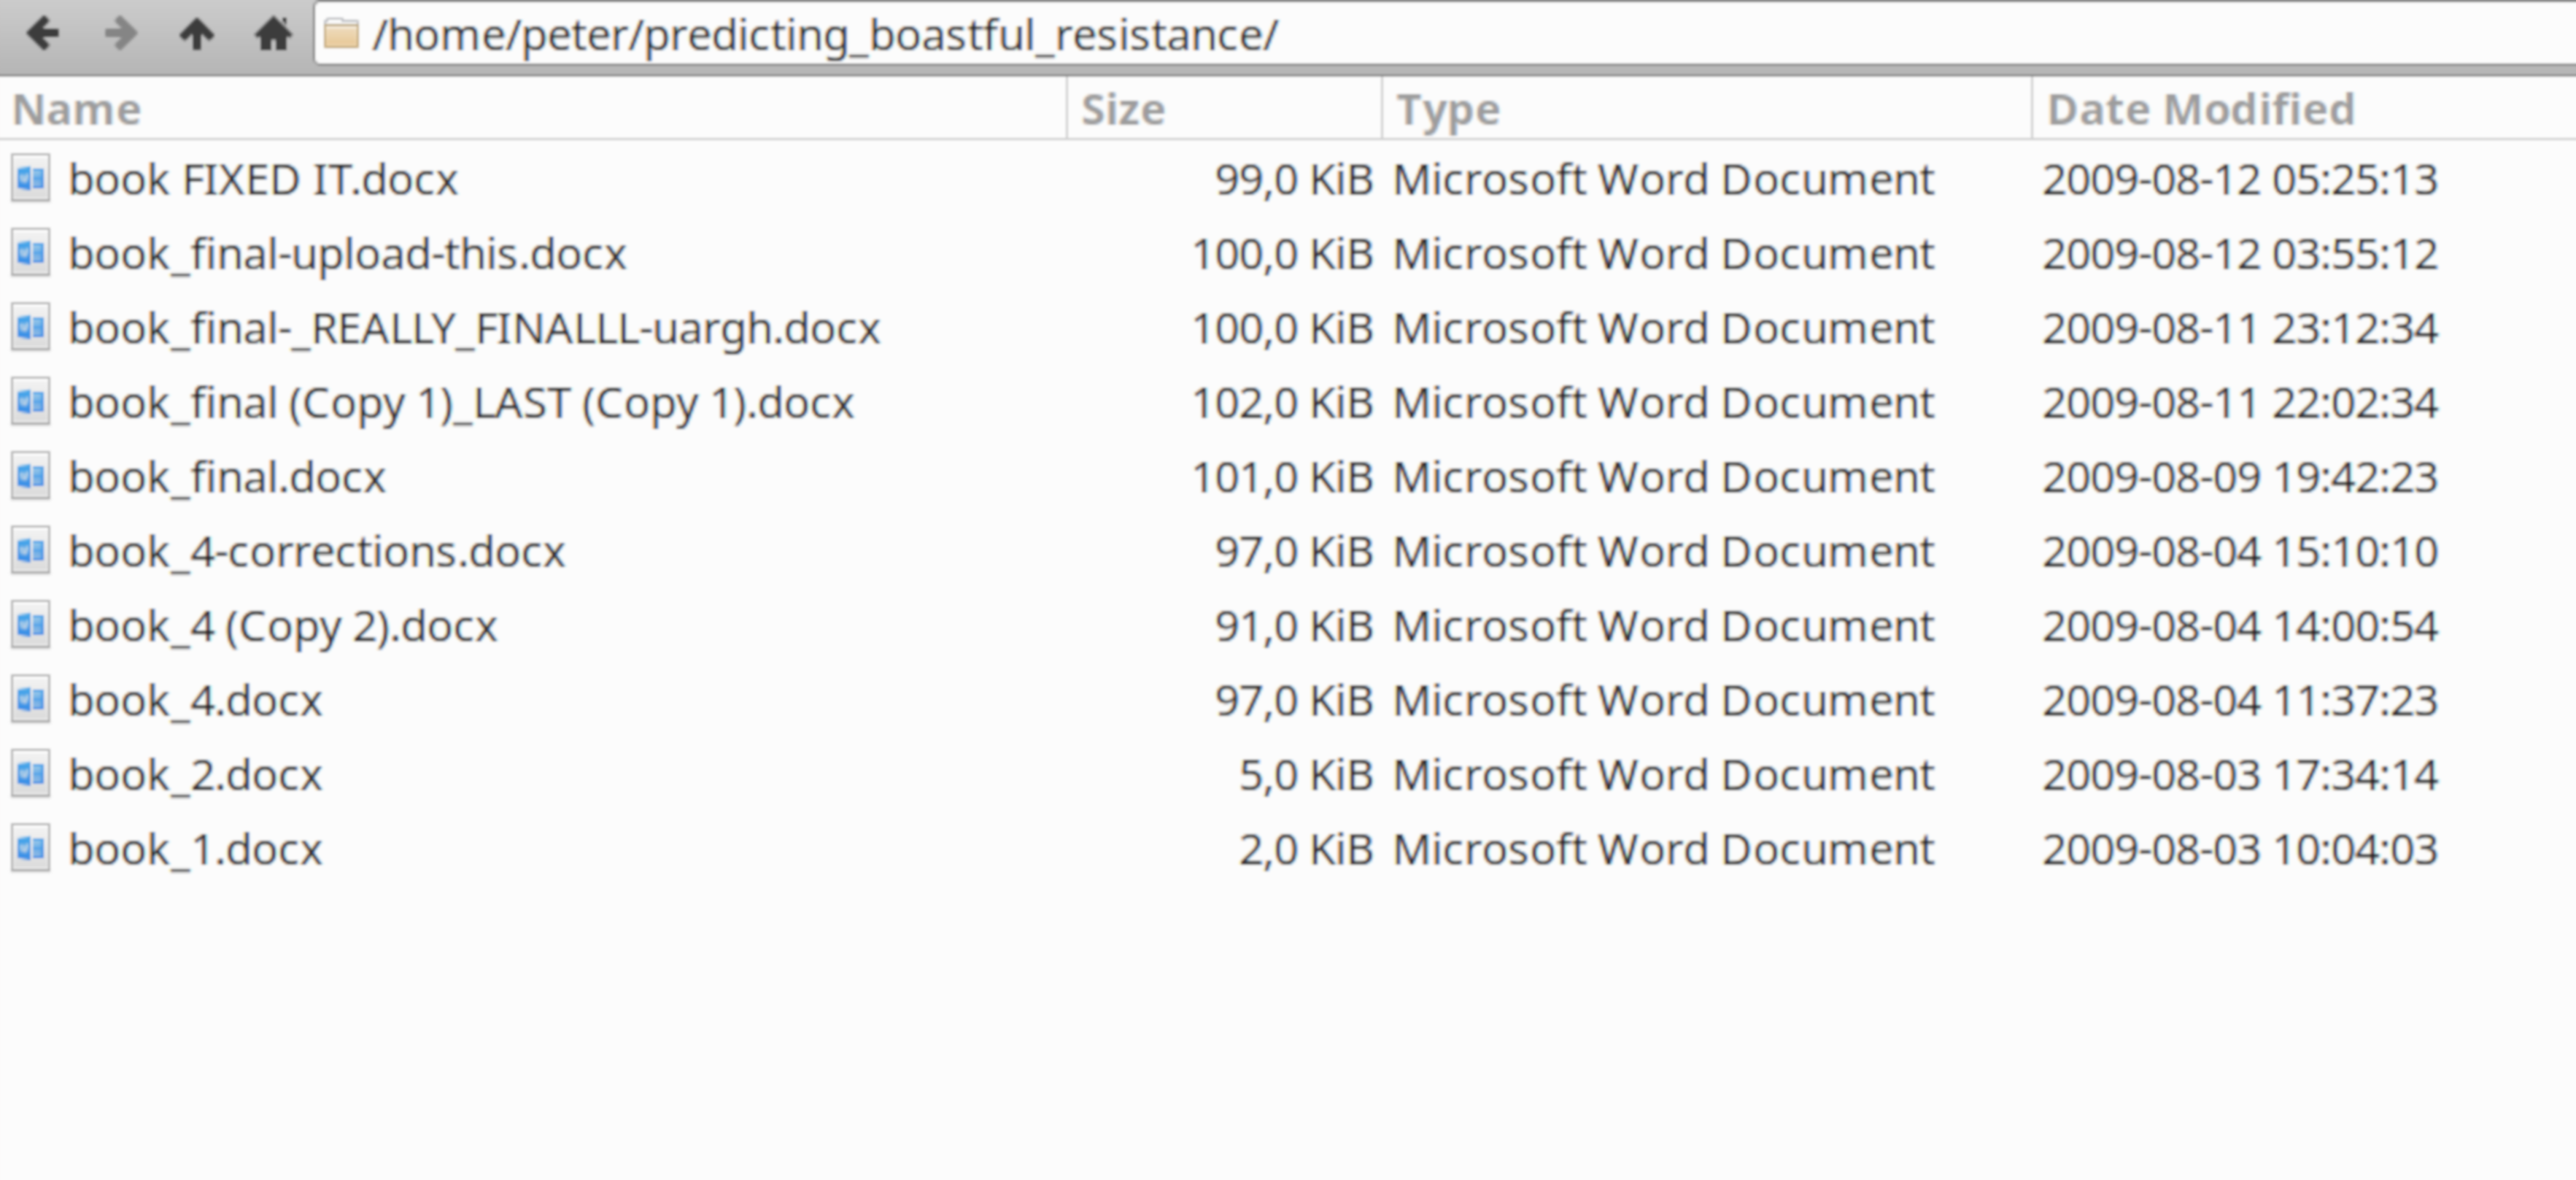
\includegraphics[width=\textwidth]{images/screenshot-ugly-filenames-1.png}
    \end{textblock*}
    \only<2->{
        \begin{textblock*}{\textwidth}(10pt, 0.85\textheight)
            If you don't see the problem here, read this:
            \href{http://phdcomics.com/comics/archive.php?comicid=1531}{http://phdcomics.com/comics/archive.php?comicid=1531}
        \end{textblock*}
    }
\end{frame}


\begin{frame}[fragile]{GIT: Chronological order}
    \begin{textblock*}{\textwidth}(10pt, 50pt)
        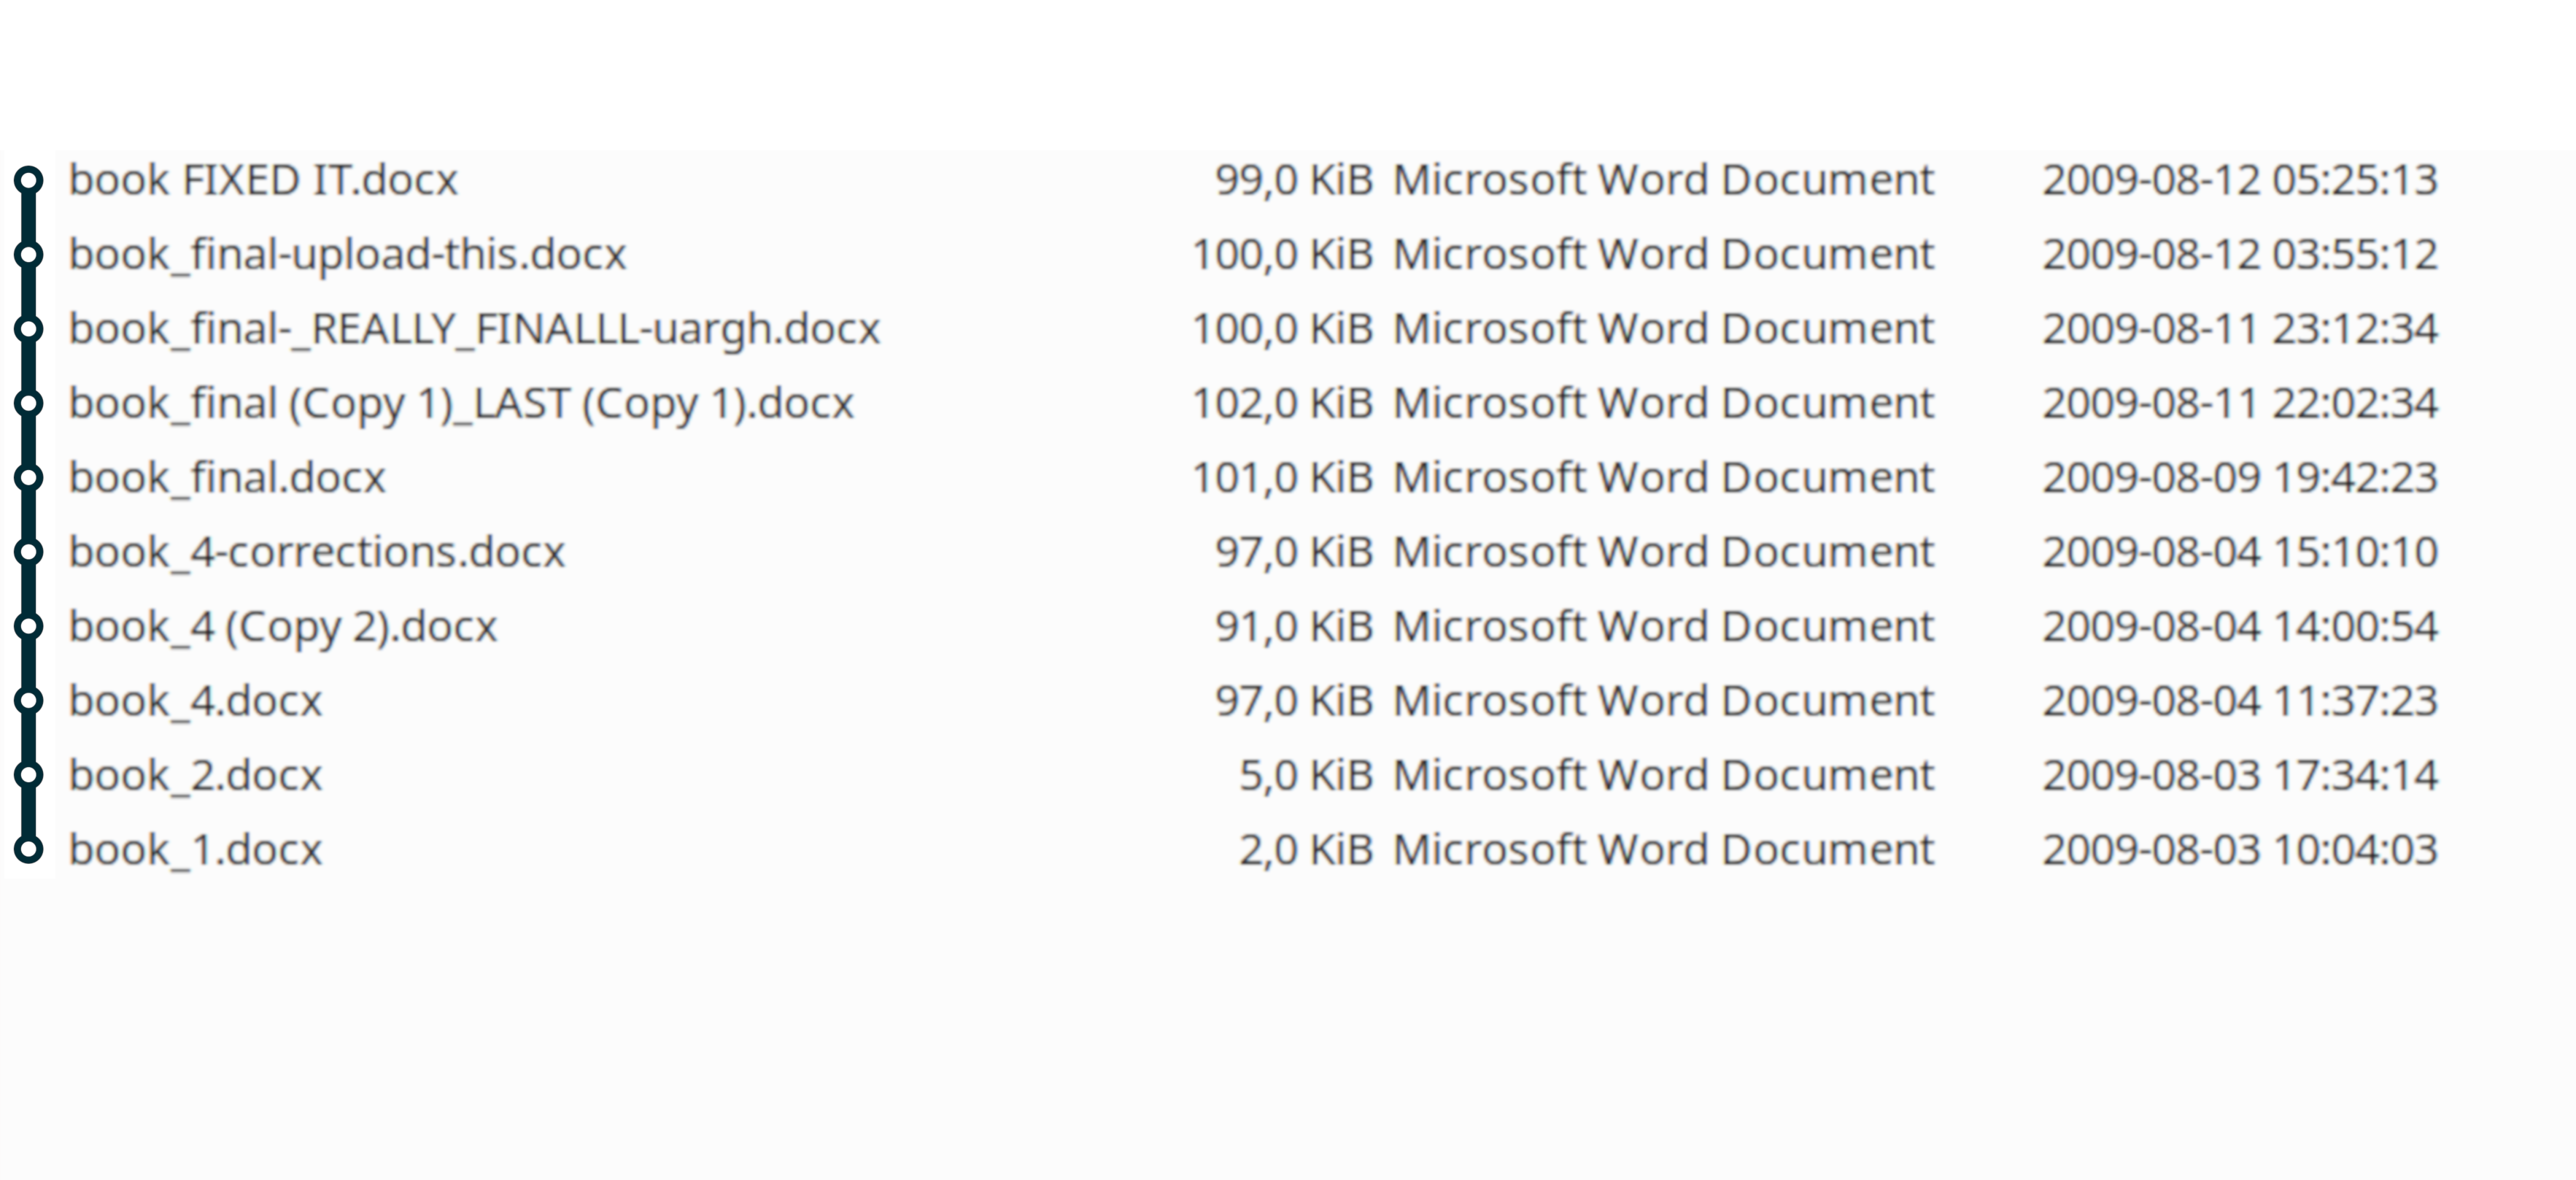
\includegraphics[width=\textwidth]{images/screenshot-ugly-filenames-2.png}
    \end{textblock*}
\end{frame}


\begin{frame}[fragile]{GIT: Describe what really happened}
    \begin{textblock*}{\textwidth}(10pt, 50pt)
        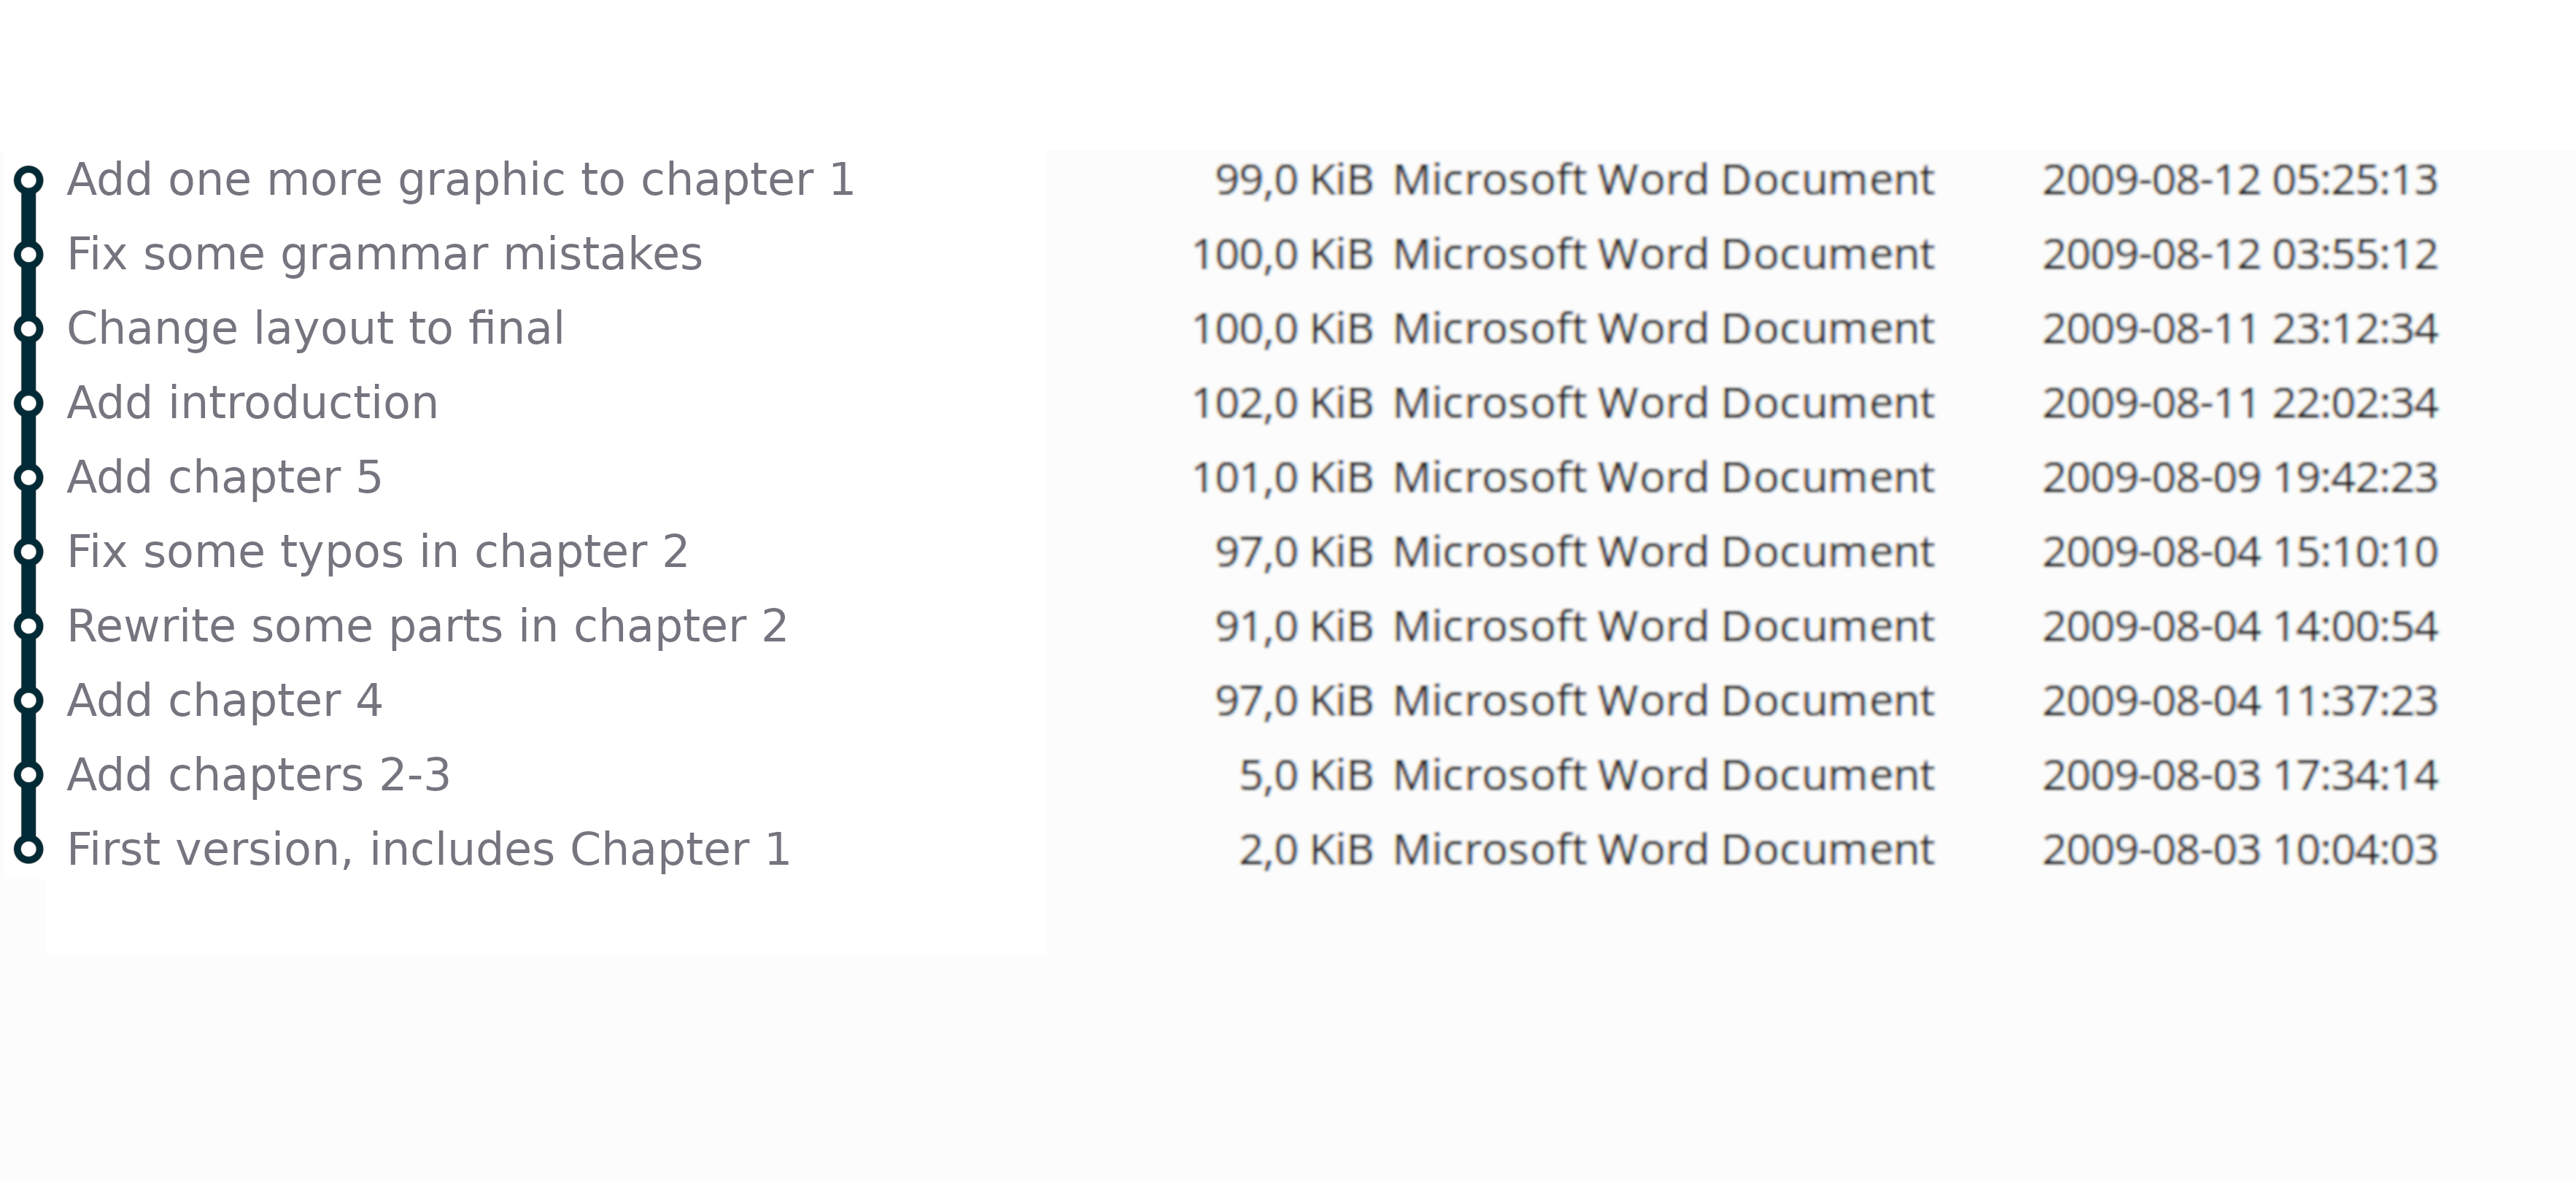
\includegraphics[width=\textwidth]{images/screenshot-ugly-filenames-3.png}
    \end{textblock*}
\end{frame}


\begin{frame}[fragile]{GIT: Authorship is important for collaboration}
    \begin{textblock*}{\textwidth}(10pt, 50pt)
        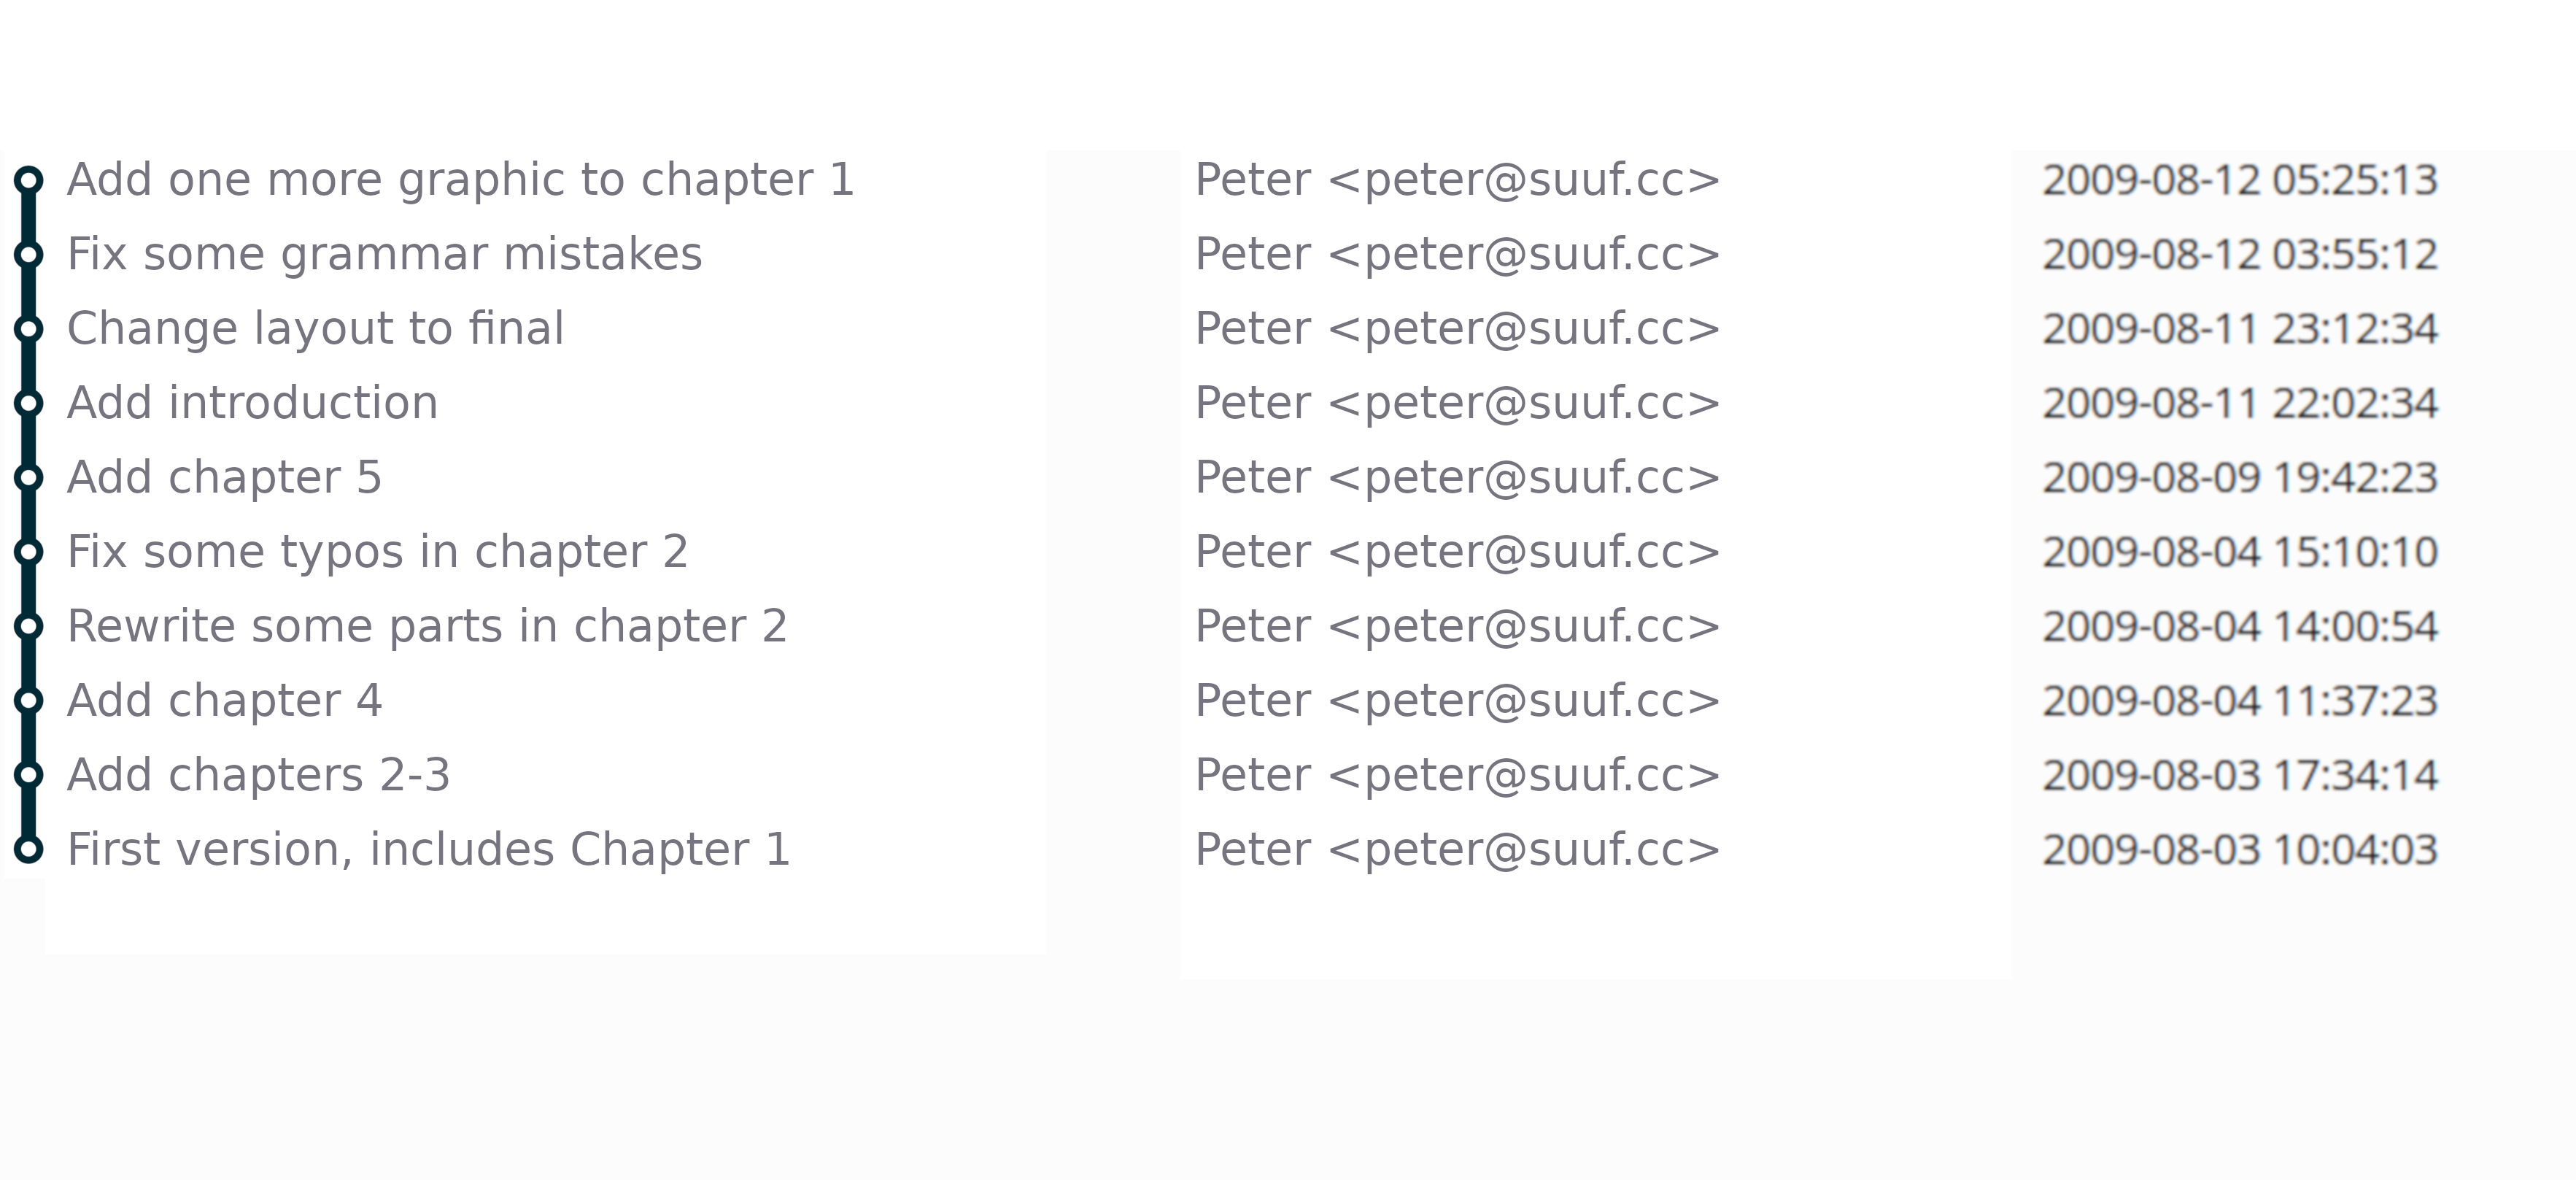
\includegraphics[width=\textwidth]{images/screenshot-ugly-filenames-4.png}
    \end{textblock*}
\end{frame}


\begin{frame}[fragile]{gitk - a simple GIT viewer}
    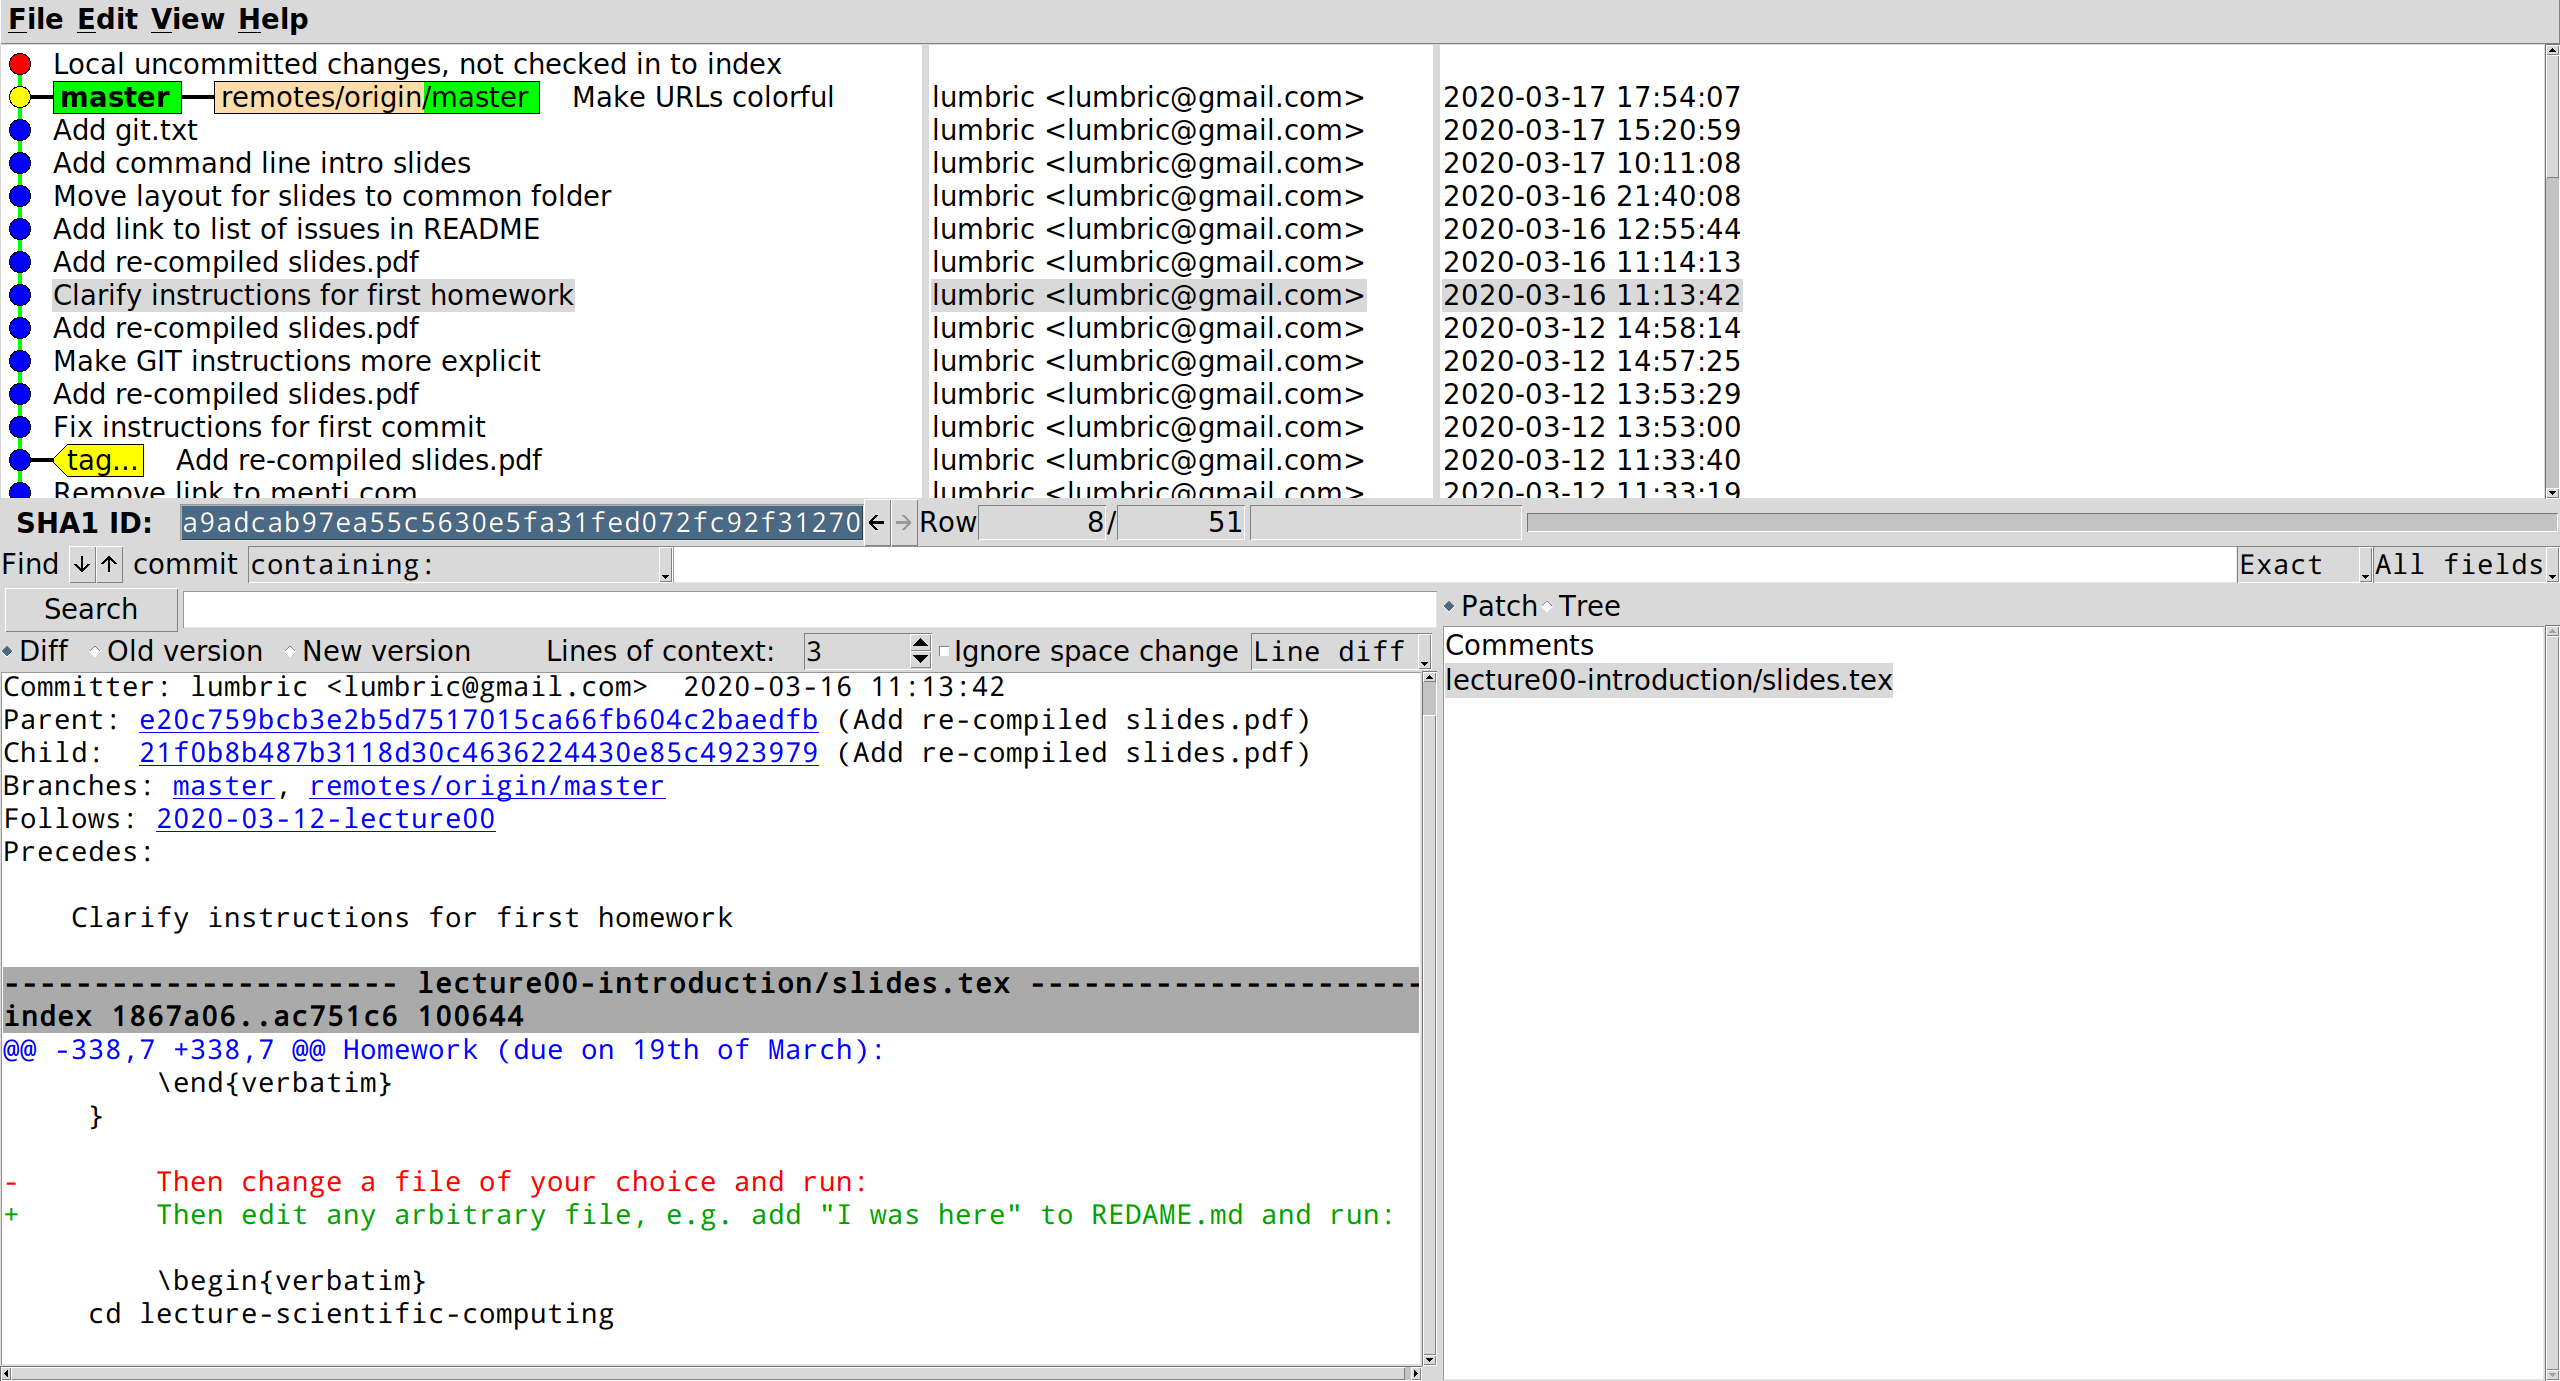
\includegraphics[width=\textwidth]{images/gitk-screenshot.png}
\end{frame}


\begin{frame}[fragile]{gitk - a simple GIT viewer}
    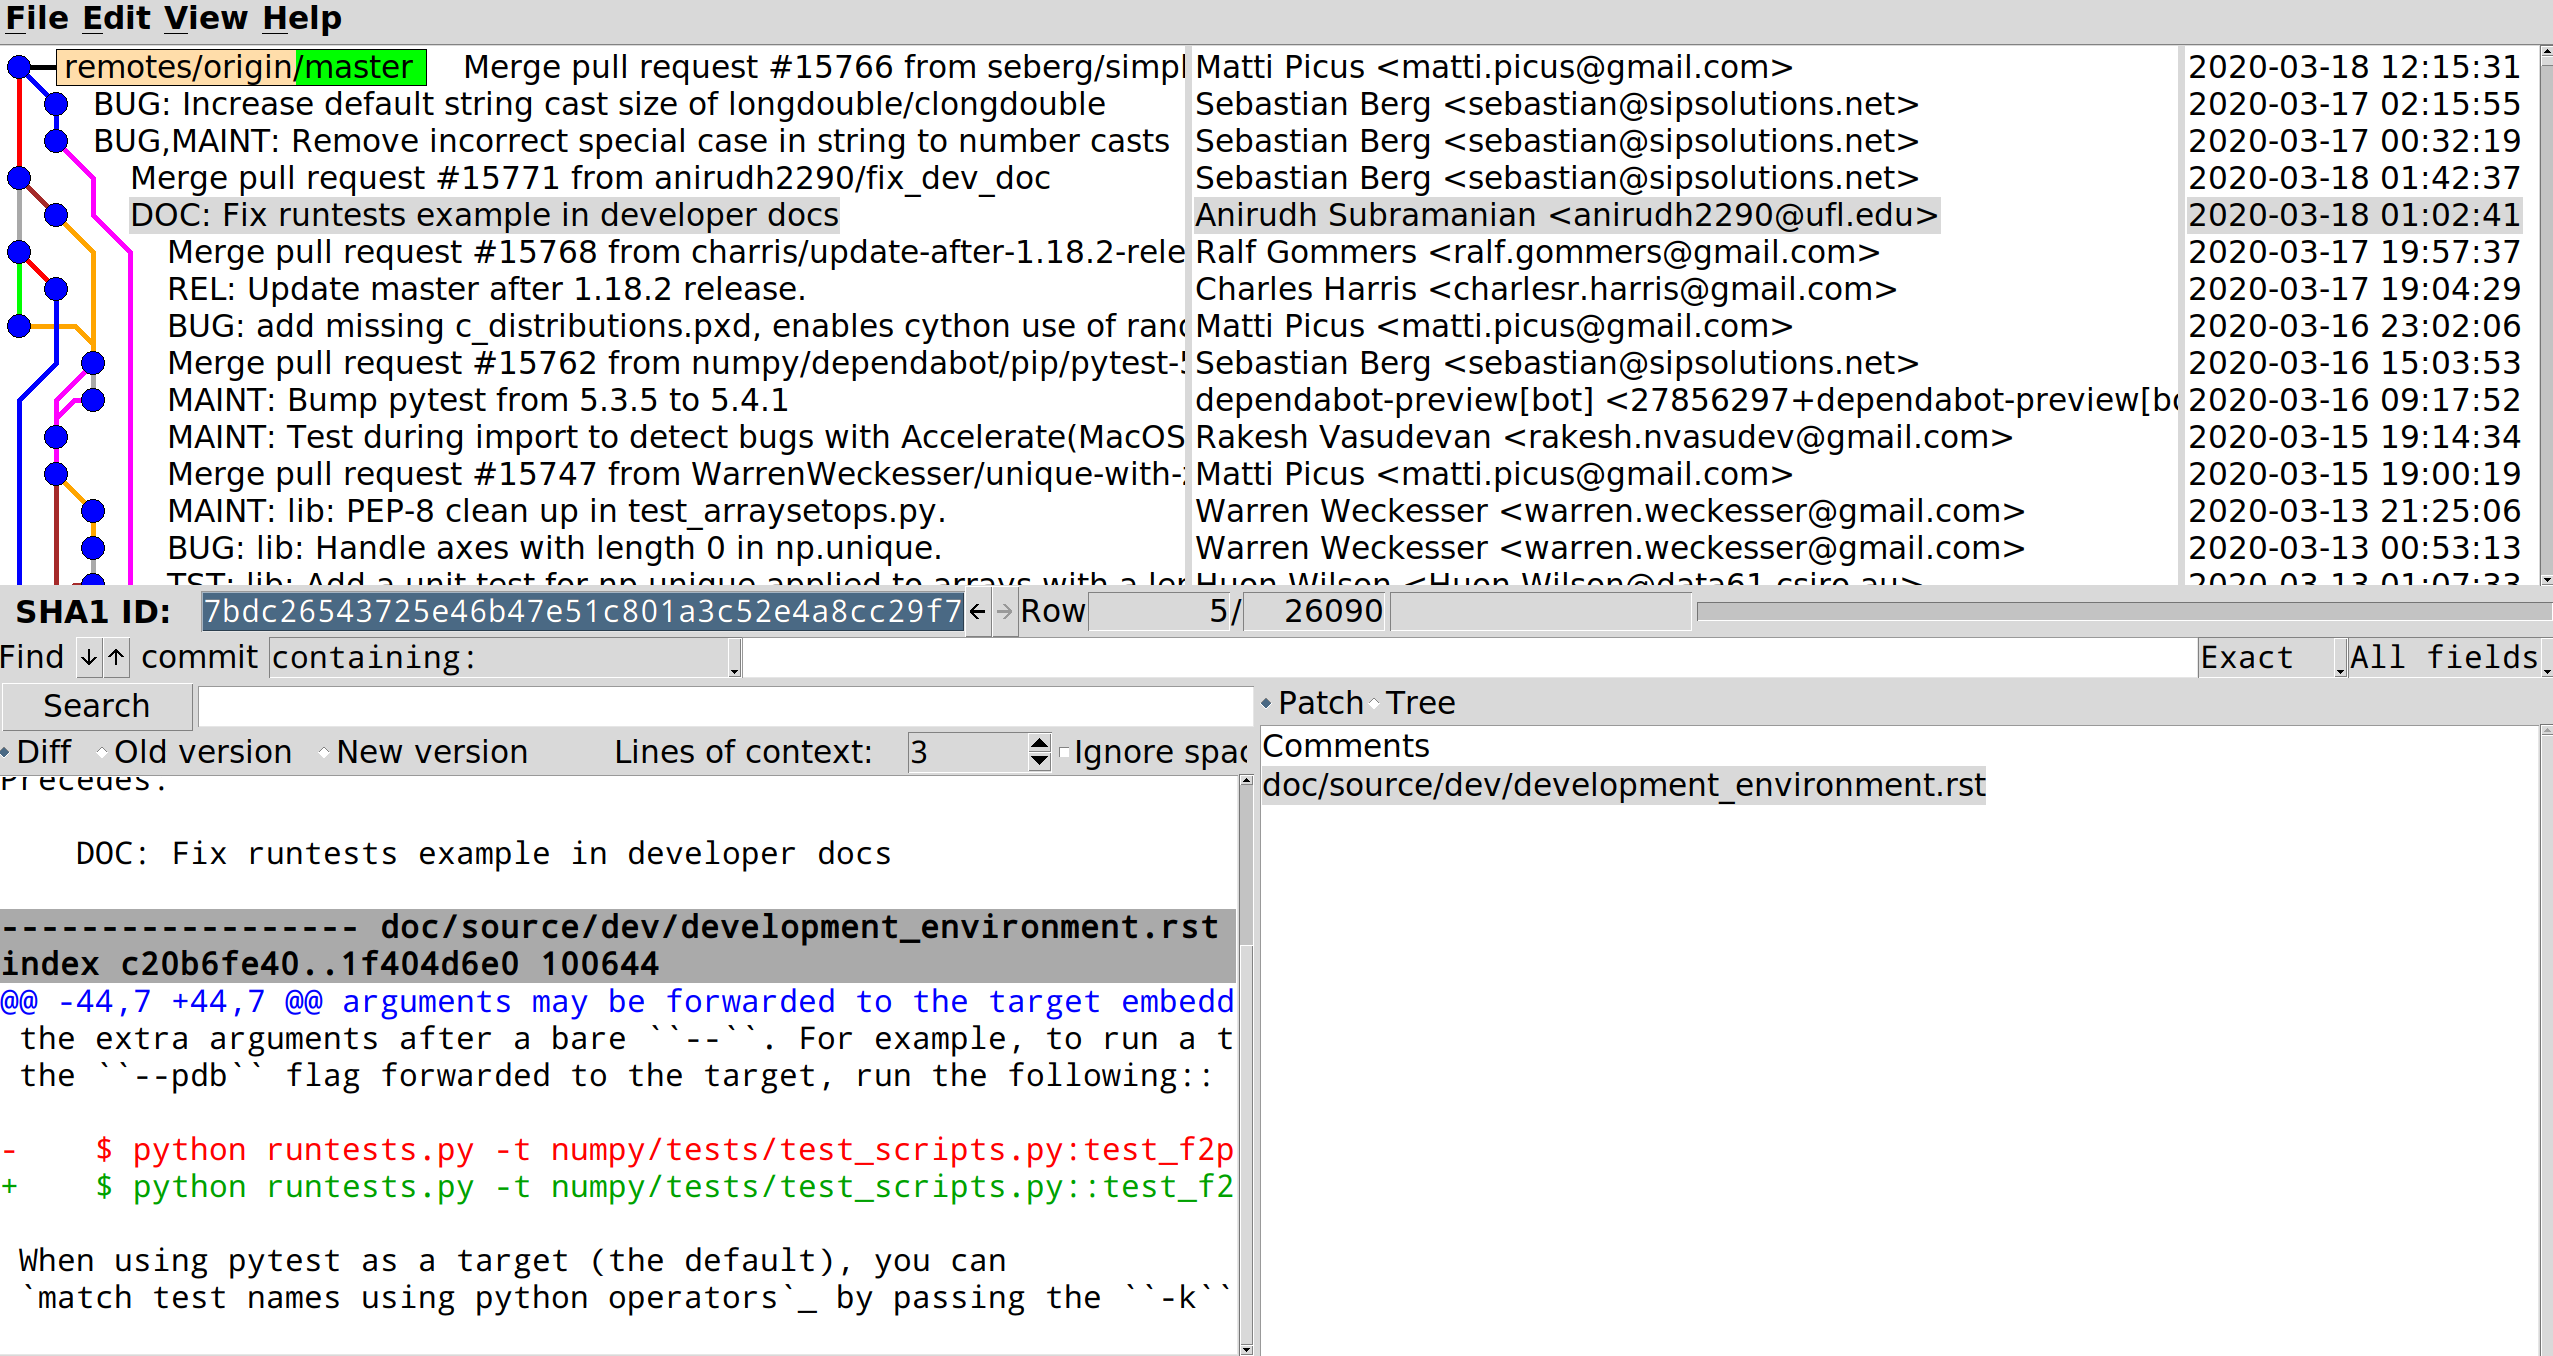
\includegraphics[width=\textwidth]{images/gitk-screenshot-numpy.png}
\end{frame}


\begin{frame}{Merging two different versions of a file}
    \begin{center}
        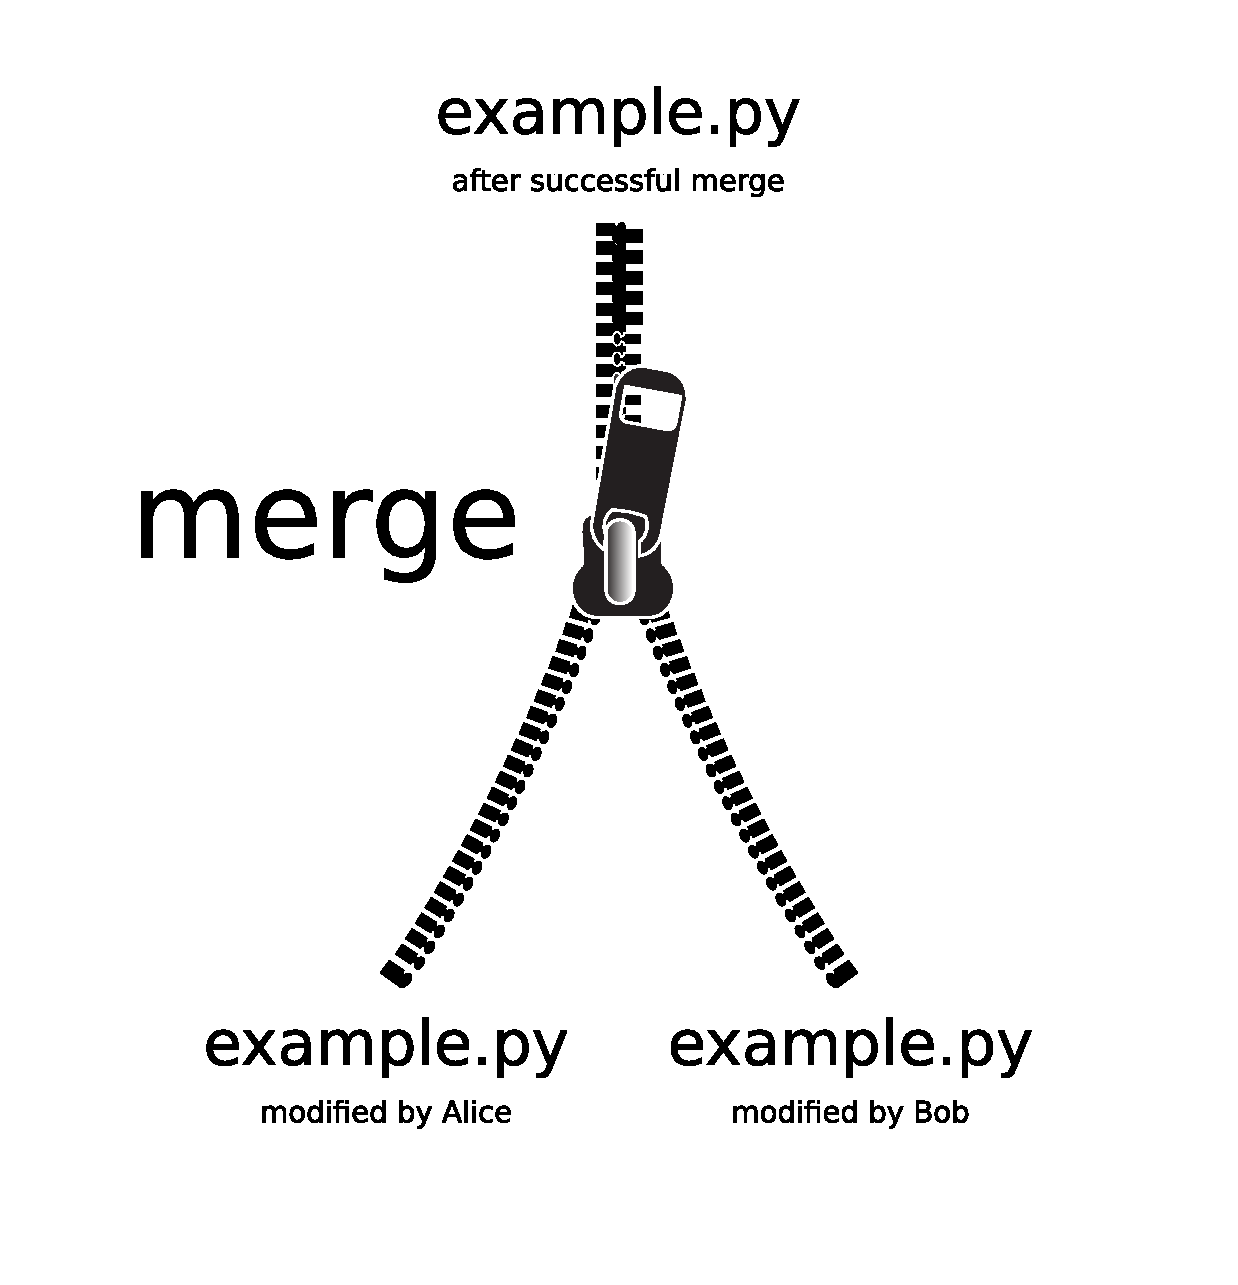
\includegraphics[height=\textheight]{images/merge.pdf}
    \end{center}
\end{frame}


\begin{frame}[fragile]{git blame}
    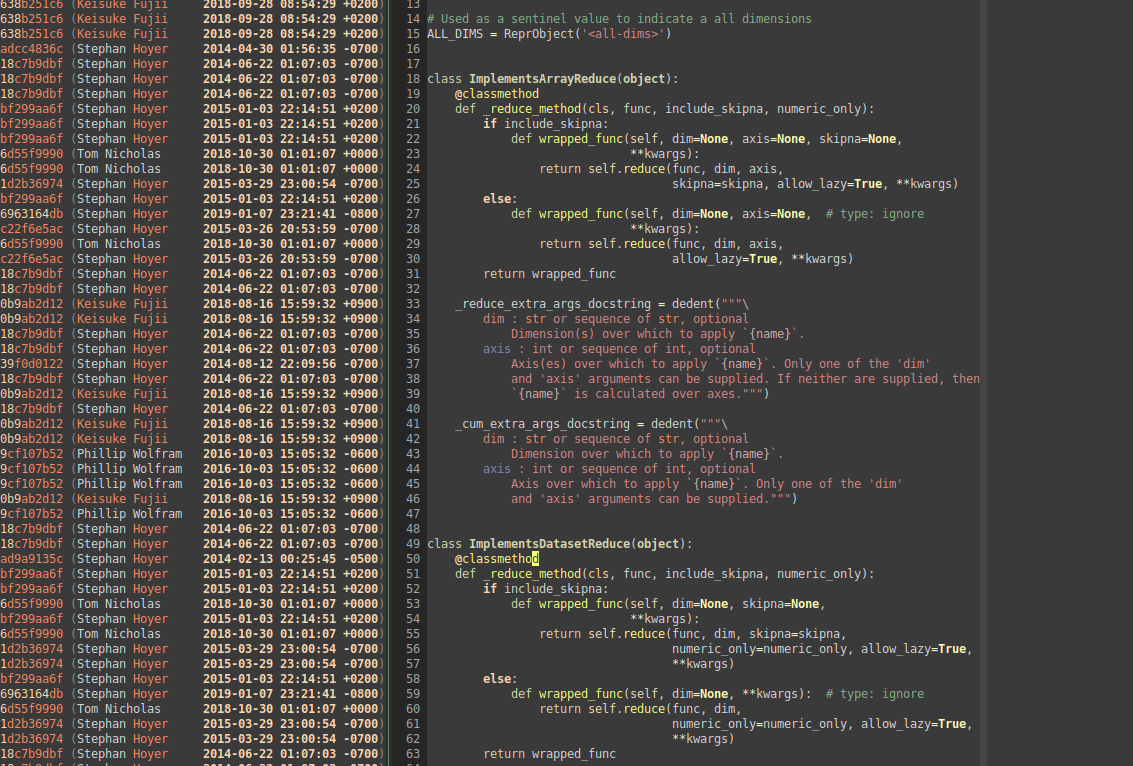
\includegraphics[width=\textwidth]{images/git-blame-screenshot.png}
\end{frame}


\begin{frame}[fragile]{git blame}
    \begin{center}
        % whut? why do we need 0.9 here?
        
\includegraphics[height=0.85\textheight]{images/git-blame2.jpg}
    \end{center}
    \vfill\pause
    {\tiny Source: http://geek-and-poke.com/geekandpoke/2013/11/24/simply-explained}
\end{frame}


\begin{frame}[fragile]{Github more popular than GIT}
    
\includegraphics[width=\textwidth]{images/git-bisect.pdf}
\end{frame}


\begin{frame}[fragile]{Github more popular than GIT}
    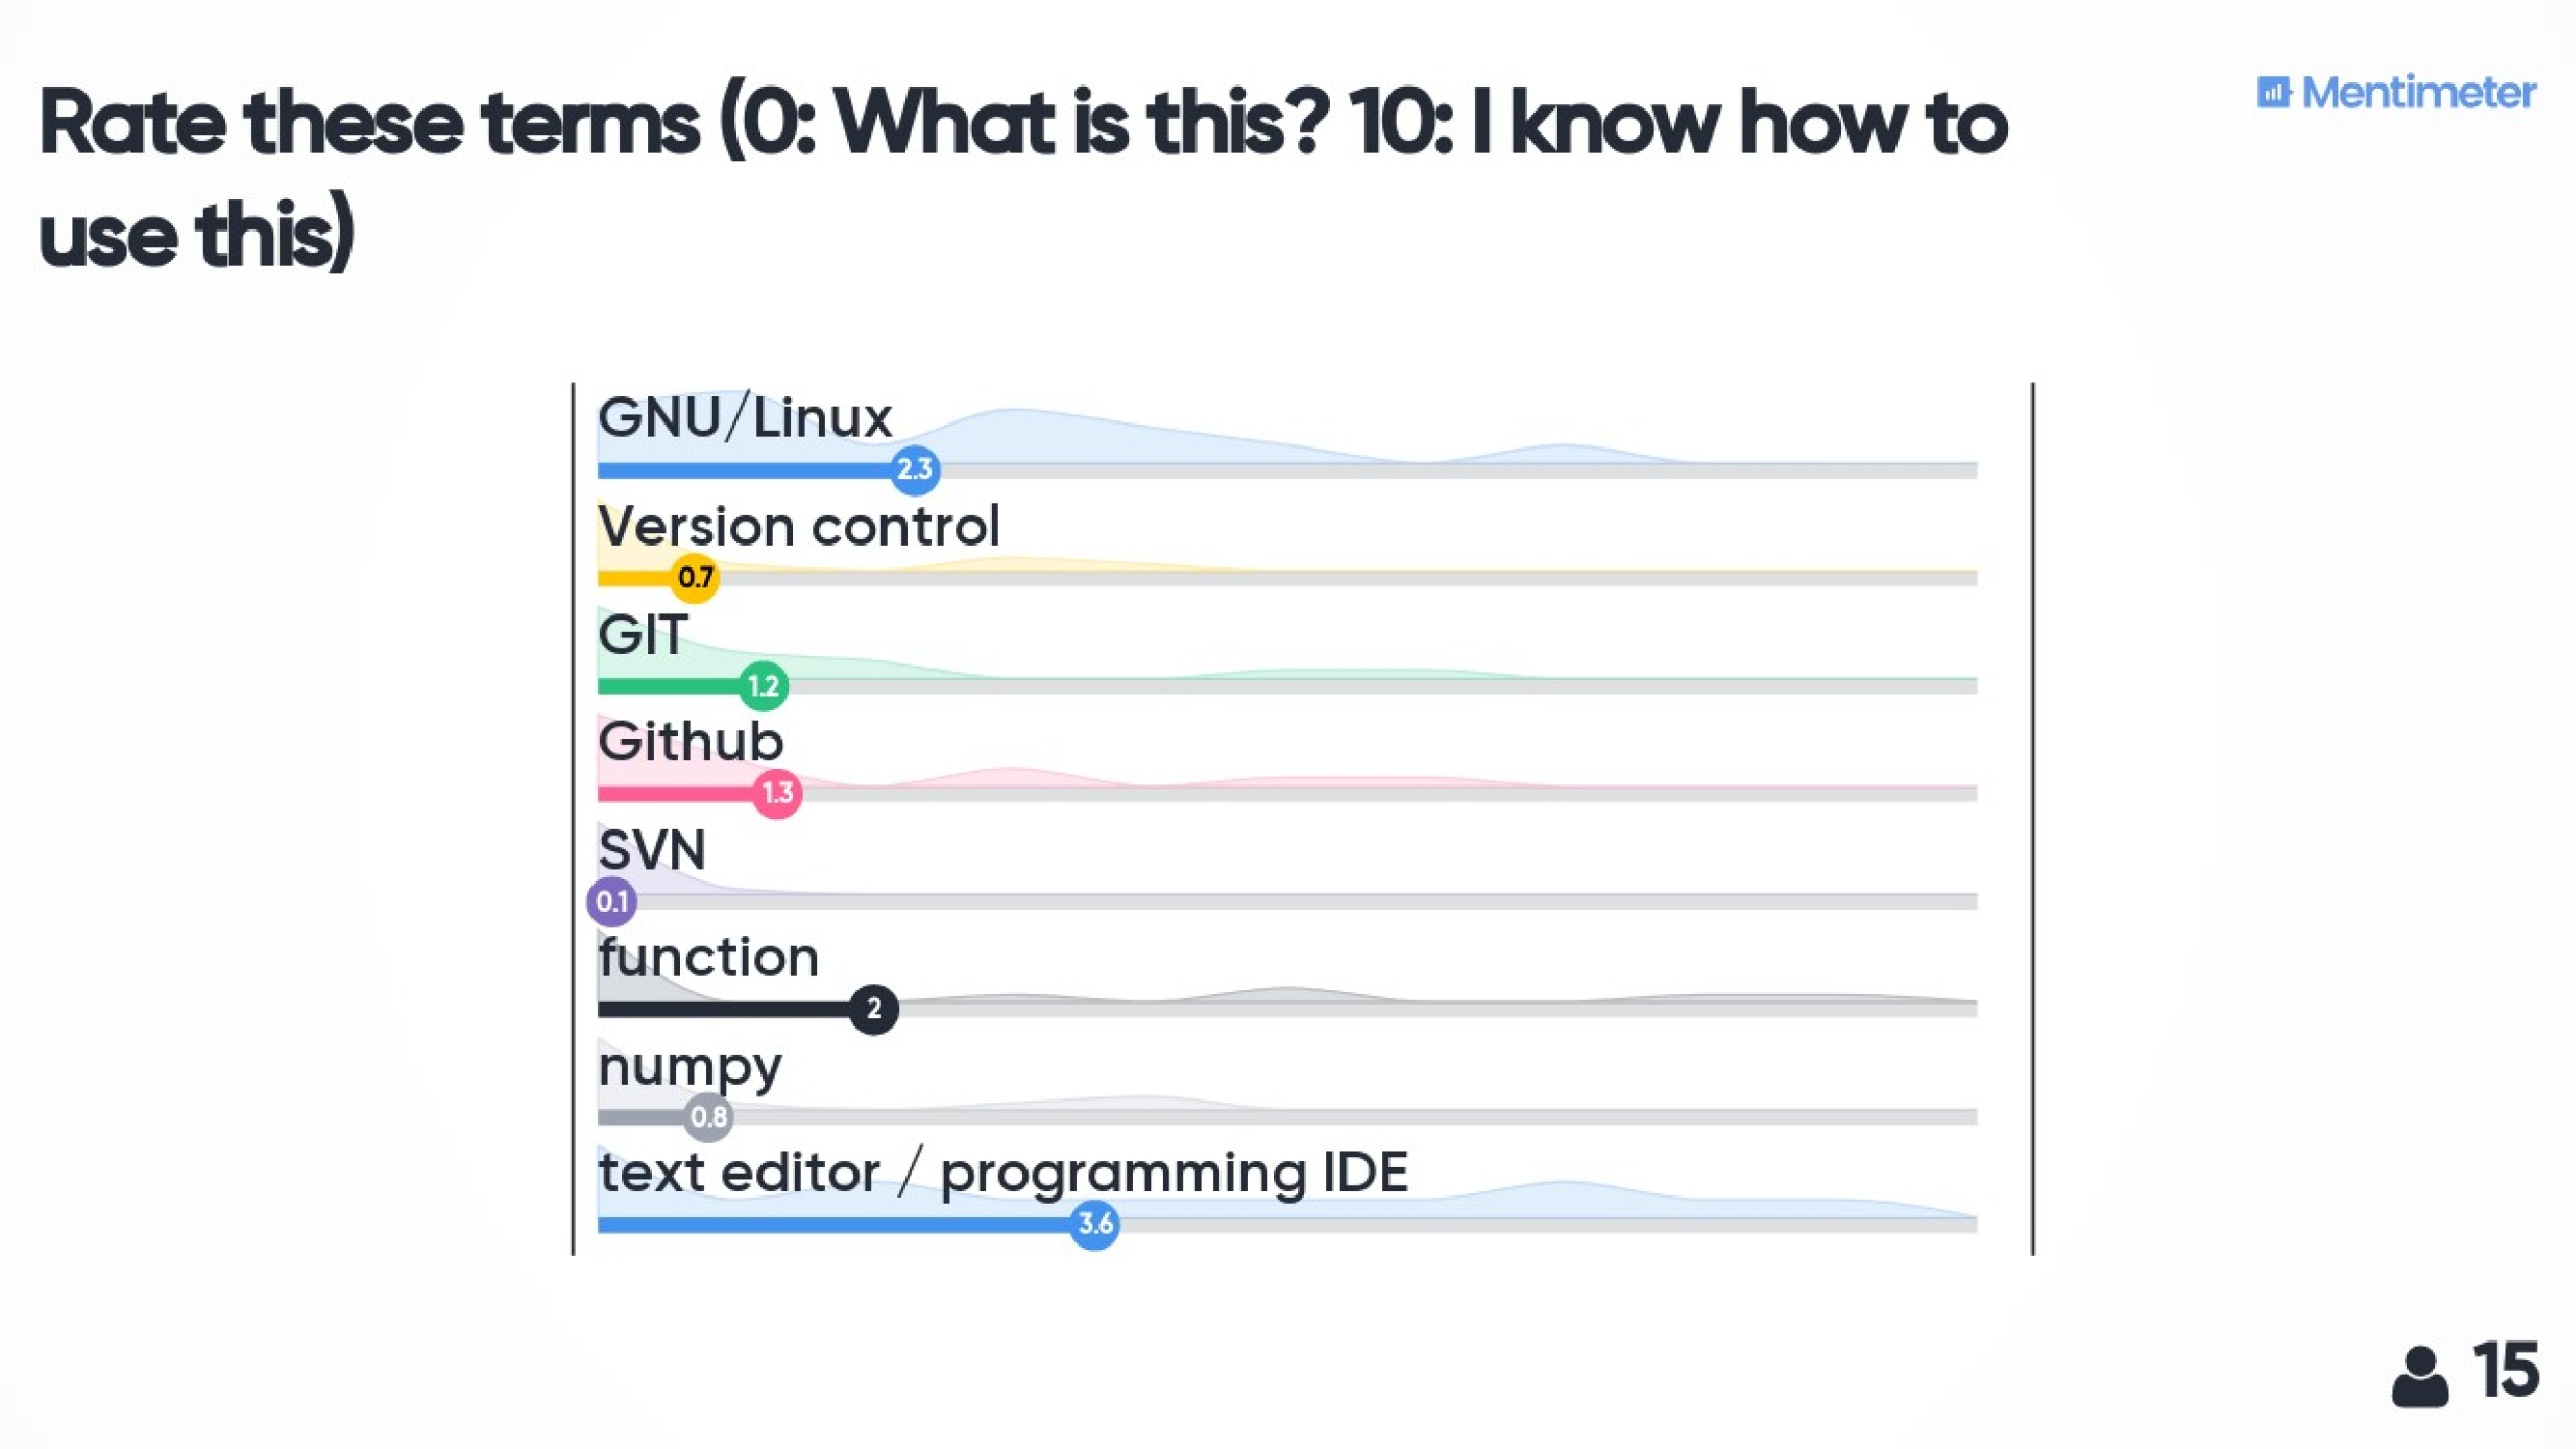
\includegraphics[width=\textwidth]{images/github-more-popular-than-git.pdf}
\end{frame}


\begin{frame}[fragile]{Github}
    Some things worth noting about the
    \href{https://github.com/inwe-boku/lecture-scientific-computing/}{Github web-interface}:
    \begin{itemize}
        \item the \verb|README.md| should give a quick intro or more complete documentation
        \item stars, watchers and forks and when the last commit are good indicators for quality
        \item by the way: if you want, watch our repository to get mail notifications if some body
            posts a question in the issue tracker
            (\href{https://help.github.com/en/github/receiving-notifications-about-activity-on-github/about-notifications}{more about watching repositories})
        \item repository settings: permissions, enable/disable features (bug tracker, wiki)
        \item license says how you are allowed to use the code
        \item Github actions allow to run code (build jobs) on Githubs servers after each commit
            (\href{https://github.com/inwe-boku/lecture-scientific-computing/actions/runs/57614853}{example})
    \end{itemize}

    \pause
    \bigskip
    Example user page:\\
    \href{https://github.com/gvanrossum}{https://github.com/gvanrossum}
\end{frame}


\begin{frame}[fragile]{GIT: Why?}
    \begin{itemize}
        \item GIT as solution for versioning files\pause
            \begin{itemize}
                \item changes ("commits") can be reverted also individually
                \item major versions (branches) can be maintained individually, changes (e.g. bug
                    fixes) applied
                \item splitting work into small parts, helps to keep an overview of changes, but
                    also to find bugs (git blame, git bisect)
            \end{itemize}
            \pause
        \item GIT as solution for collaboration\pause
            \begin{itemize}
                \item multiple developers can work on code at the same time independently and then
                    merge changes into one version
                \item work is split into readable and consistent parts, which allows code review by
                    other developers
            \end{itemize}
            \pause
        \item GIT for distributing software/code\pause
            \begin{itemize}
                \item Github is the main platform for hosting opensource code
                \item libraries and applications can often be installed directly from Github
                \item Github issues, Pull requests and stars allow interaction with the community
            \end{itemize}
    \end{itemize}
\end{frame}


\begin{frame}[fragile]{GIT: What?}
    \begin{itemize}
        \item versions are connected via a tree-like graph, each node is a commit (=one version of
            the entire project)\pause
        \item think of the commit as change ("patch") to the previous version, especially when
            writing the commit message\pause
        \item there are operations on the tree of commits: branch, rebase, cherry-pick, merge,
            copy commits to/from Github (= push/pull)
    \end{itemize}
\end{frame}


\begin{frame}[fragile]{GIT: How?}
    \begin{itemize}
        \item command line (that's how we will do it)
        \item GUIs (e.g. gitk), IDE integration
        \item API (eg. Python or commit sha1 on first page of slides)
    \end{itemize}
\end{frame}

\begin{frame}[fragile]{GIT is difficult... :(}
    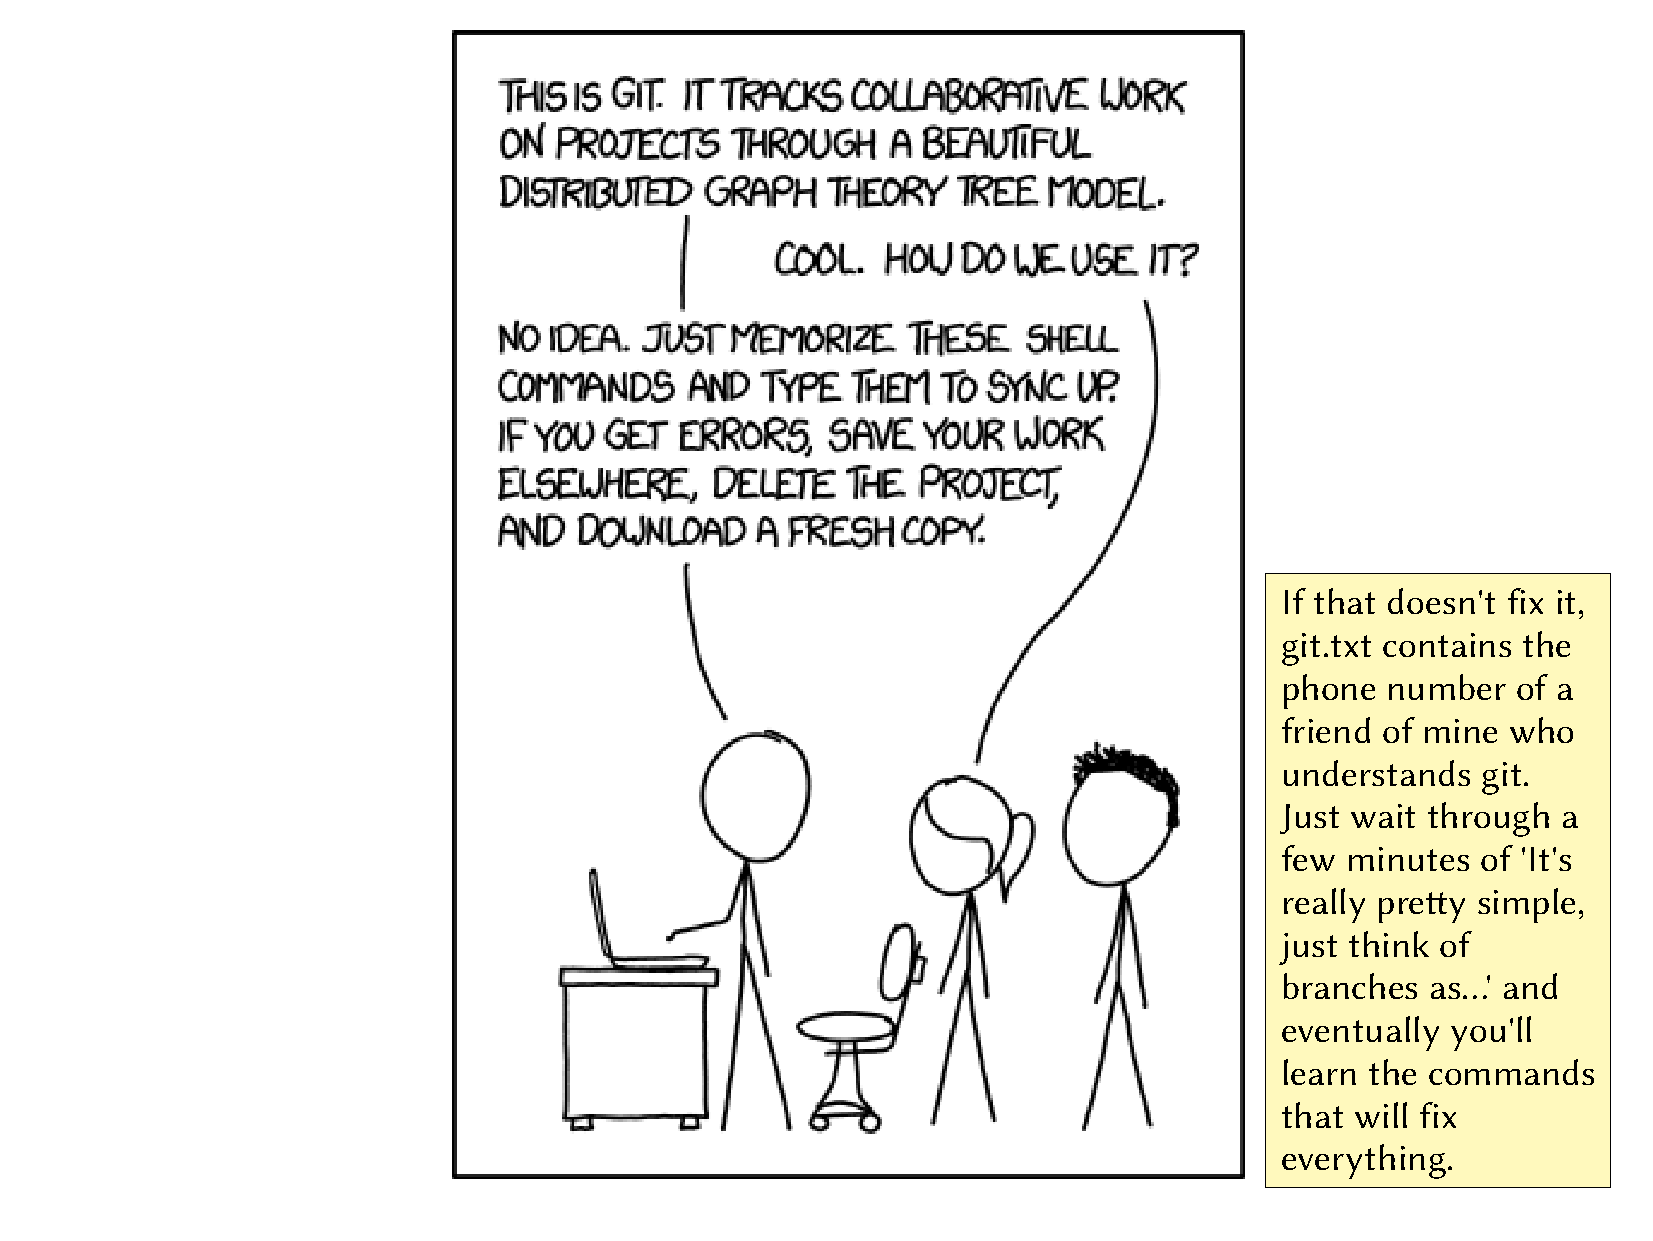
\includegraphics[width=0.84\textwidth]{images/xkcd-git-is-hard.pdf}
    \vfill
    {\tiny Source:
        \href{https://xkcd.com/1597kjA}{https://xkcd.com/1597}
    }
\end{frame}

% TODO
% - add fake git man pages
% - add link to svn is better than git

\begin{frame}[fragile]{GIT terminology}
    \begin{itemize}
        \item version control system: a tool like GIT (alternatives: hg, SVN, ...)
        \item repository: a folder with files under version control, the complete history is
            stored in the subfolder \verb|.git|
        \item commit: one version of the repository or equivalently the change made in this
            version
        \item commit message: a short message describing what has been changed in the commit
            and if not obvious, why it was a good idea to change it
        \item working directory (or working tree): the folder where files can be edited (don't
            confuse it with the commit history, which is tree-like!)
    \end{itemize}
\end{frame}


\begin{frame}[fragile]{Github: things to know}
    \begin{itemize}
        \item fork: copy a GIT repository from a Github account to your own account, typically in
            order to get write permissions in the repository
        \item pull request: ask the original owner to copy commits from the forked repository
            back to the original repository
        \item repository collaborators: to allow others to write to your repository,
            invite them as collaborator via the Github webpage of the repository:\\
            Settings/Manage access/Invite a collaborator
    \end{itemize}
\end{frame}


\begin{frame}[fragile]{GIT commands}
    \begin{itemize}
        \item Copy a GIT repository from Github to your computer:\\
            \verb|git clone https://github.com/lumbric/git-games/|
        \item Add a new file to the repository:\\
            \verb|git add path/to/file|
        \item Commit a file, i.e. record the current version for the GIT history:
            \verb|git commit path/to/file|
        \item Which changes/files have not yet been committed:\\
            \verb|git status|
        \item Copy new commits from local machine to Github:\\
            \verb|git push|
        \item Copy new commits from Github to local machine:\\
            \verb|git pull|
    \end{itemize}
\end{frame}


\begin{frame}[fragile]{GIT display changes}
    \begin{itemize}
        \item gitk has a nice tree viewer, but looks a bit old fashioned
        \item Github has a nice web interface, but no tree viewer
        \item on the command line use \verb|git show| or \verb|git diff|
    \end{itemize}
\end{frame}


\begin{frame}[fragile]{Discuss questions collected as homework}

    Questions in etherpad:\\
    \href{https://yourpart.eu/p/lecture-scientific-computing}{https://yourpart.eu/p/lecture-scientific-computing}
\end{frame}


\begin{frame}[fragile]{Bonus: Branches, merges and conflicts}
    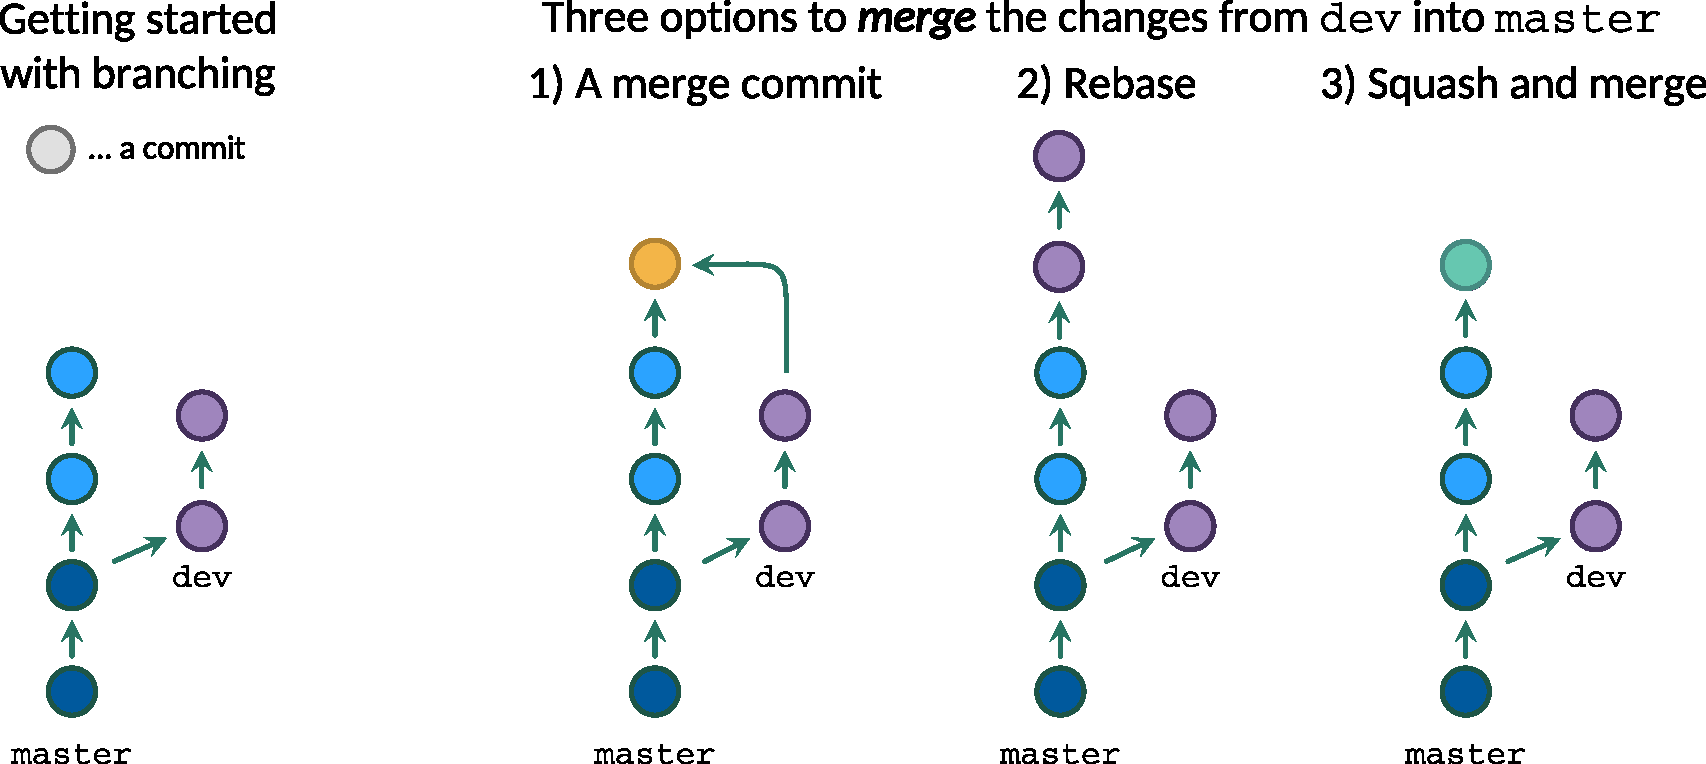
\includegraphics[width=\textwidth]{images/merging-diagram.pdf}
\end{frame}

\begin{frame}[fragile]{Bonus: Merge conflicts}
    \begin{itemize}
        \item You run \verb|git pull| or \verb|git merge| or \verb|git rebase| and then see the error:
            {\small
            \begin{verbatim}CONFLICT (content): Merge conflict in example.py
Automatic merge failed; fix conflicts and then commit the result.\end{verbatim}\pause
            }
        \item Look for lines like these in \verb|example.py|:
\begin{verbatim}
<<<<<<< HEAD
some change
=======
some other change
>>>>>>> other\end{verbatim}
        \item edit the file, delete the markers and the parts you don't need\pause
        \item run \verb|git add example.py| and \verb|git commit|
    \end{itemize}
\end{frame}


\begin{frame}[fragile]{Bonus: GIT workflow}
    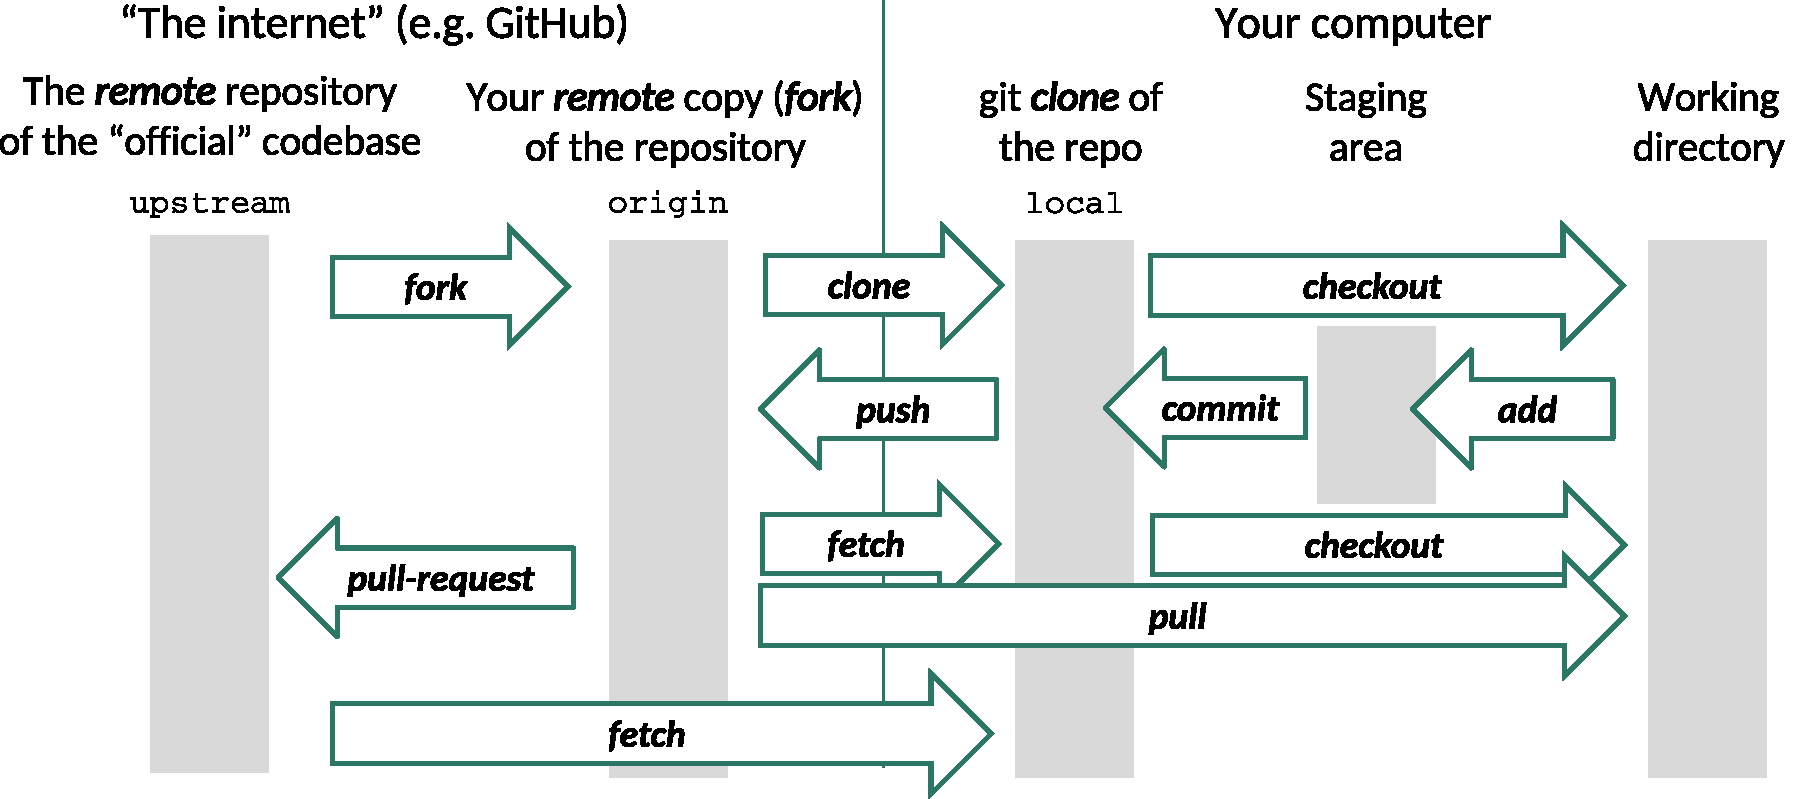
\includegraphics[width=\textwidth]{images/git-workflow.pdf}
    \pause
    \vfill
    {\tiny Source:
    \href{https://data.ene.iiasa.ac.at/teaching/_static/osesm_summer2019/Lecture_1.pdf}{Slides} for
    \href{https://data.ene.iiasa.ac.at/teaching/#tu-vienna-summer-semester-2019-370-062}{Open Source Energy System Modeling}
    by \href{github.com/danielhuppmann}{Daniel Huppmann}, CC-BY 4.0
    }
\end{frame}


\begin{frame}[fragile]{Bonus: More topics}
    Also good to know, but probably beyond the scope of this lecture today...
    \begin{itemize}
        \item what is the GIT sha1 / hash?
        \item licenses and open source
        \item the \verb|.gitignore| file
        \item different ways of reverting, see also \href{https://ohshitgit.com/}{ohshitgit.com}
        \item what does \verb|git add| actually do?
        \item how does a pull request work exactly?
    \end{itemize}
\end{frame}


\section{Exercise}

\begin{frame}[fragile]{Exercise}
    \begin{itemize}
        \item Go to \href{https://github.com/lumbric/git-games/}{https://github.com/lumbric/git-games/}
        \item read the instructions in \verb|README.md| and choose a game (e.g. tic-tac-toe)
        \item follow the instructions in the \verb|README.md| of the game you choose, e.g.
            \href{https://github.com/lumbric/git-games/tree/master/tic-tac-toe#how-to-play}{Tic-tac-toe}

    \end{itemize}
\end{frame}


\section{Homework assignment}

\begin{frame}[fragile]{Homework assignment}
    \begin{itemize}
        \item decide one maintainer for each group
        \item maintainer only: fork the exercise repository\\
            \href{https://github.com/inwe-boku/homework-scientific-computing}{https://github.com/inwe-boku/homework-scientific-computing}
        \item add other group members as collaborators to the forked repository in Github
        \item one group member only: create a hello world program or some other simple file with
            code or text file, add and commit it and push it
        \item other group members: change something (e.g. add another print statement) and commit
          the changes and push them to Github
        \item bonus points if you manage to get a merge-conflict on purpose and resolve it correctly
    \end{itemize}
\end{frame}

\end{document}
